% Options for packages loaded elsewhere
\PassOptionsToPackage{unicode}{hyperref}
\PassOptionsToPackage{hyphens}{url}
%
\documentclass[
]{article}
\usepackage{amsmath,amssymb}
\usepackage{iftex}
\ifPDFTeX
  \usepackage[T1]{fontenc}
  \usepackage[utf8]{inputenc}
  \usepackage{textcomp} % provide euro and other symbols
\else % if luatex or xetex
  \usepackage{unicode-math} % this also loads fontspec
  \defaultfontfeatures{Scale=MatchLowercase}
  \defaultfontfeatures[\rmfamily]{Ligatures=TeX,Scale=1}
\fi
\usepackage{lmodern}
\ifPDFTeX\else
  % xetex/luatex font selection
\fi
% Use upquote if available, for straight quotes in verbatim environments
\IfFileExists{upquote.sty}{\usepackage{upquote}}{}
\IfFileExists{microtype.sty}{% use microtype if available
  \usepackage[]{microtype}
  \UseMicrotypeSet[protrusion]{basicmath} % disable protrusion for tt fonts
}{}
\makeatletter
\@ifundefined{KOMAClassName}{% if non-KOMA class
  \IfFileExists{parskip.sty}{%
    \usepackage{parskip}
  }{% else
    \setlength{\parindent}{0pt}
    \setlength{\parskip}{6pt plus 2pt minus 1pt}}
}{% if KOMA class
  \KOMAoptions{parskip=half}}
\makeatother
\usepackage{xcolor}
\usepackage[margin=1in]{geometry}
\usepackage{graphicx}
\usepackage{float} % allows [H] placement so figures stay exactly where they appear in the text
\makeatletter
\def\maxwidth{\ifdim\Gin@nat@width>\linewidth\linewidth\else\Gin@nat@width\fi}
\def\maxheight{\ifdim\Gin@nat@height>\textheight\textheight\else\Gin@nat@height\fi}
\makeatother
% Scale images if necessary, so that they will not overflow the page
% margins by default, and it is still possible to overwrite the defaults
% using explicit options in \includegraphics[width, height, ...]{}
\setkeys{Gin}{width=\maxwidth,height=\maxheight,keepaspectratio}
% Set default figure placement to htbp
\makeatletter
\def\fps@figure{htbp}
\makeatother
\setlength{\emergencystretch}{3em} % prevent overfull lines
\providecommand{\tightlist}{%
  \setlength{\itemsep}{0pt}\setlength{\parskip}{0pt}}
\setcounter{secnumdepth}{5} % number sections down to \subparagraph, matching the original numbering
\usepackage{titlesec}
% Give \paragraph and \subparagraph their own line (bold heading), like the other levels,
% instead of LaTeX's default run-in style, and keep them numbered.
\titleformat{\paragraph}
  {\normalfont\normalsize\bfseries}{\theparagraph}{1em}{}
\titlespacing*{\paragraph}{0pt}{2.5ex plus 1ex minus .2ex}{1ex plus .2ex}
\titleformat{\subparagraph}
  {\normalfont\normalsize\itshape}{\thesubparagraph}{1em}{}
\titlespacing*{\subparagraph}{0pt}{2.25ex plus 1ex minus .2ex}{1ex plus .2ex}
\ifLuaTeX
  \usepackage{selnolig}  % disable illegal ligatures
\fi
\IfFileExists{bookmark.sty}{\usepackage{bookmark}}{\usepackage{hyperref}}
\IfFileExists{xurl.sty}{\usepackage{xurl}}{} % add URL line breaks if available
\urlstyle{same}
\hypersetup{
  hidelinks,
  pdfcreator={LaTeX via pandoc}}

\title{\protect\hypertarget{_Hlk535482051}{}{}Tausand

Tempico Software 2.1.0

Software for Tempico TP1004 \& TP1204}
\author{}
\date{}

\begin{document}
\maketitle

\begin{figure}[H]
\centering

\includegraphics[width=4.49565in,height=2.01282in]{images/titlepage-01.png}
\label{fig:1}
\end{figure}

\begin{center}
User's manual

Rev 1.5

\today

\href{http://www.tausand.com}{www.tausand.com}
\end{center}

\newpage

{
\setcounter{tocdepth}{5}
\tableofcontents
}




\hypertarget{definitions}{%
\section{Definitions}\label{definitions}}

\hypertarget{sampling-time}{%
\subsection{Sampling time}\label{sampling-time}}

The sampling time in an experiment refers to the time window during
which data is collected. For example, if we count how many times the
laboratory door opens over the course of 2 hours, the sampling time
would be 2 hours.

\hypertarget{edge-type}{%
\subsection{Edge type}\label{edge-type}}

The edge type indicates the type of transition that the time-to-digital
converter (TDC) must use to start or stop a measurement. There are two
main types: rise edge and falling edge. An event arriving at a TDC must
be a short-duration pulse that exceeds the device\textquotesingle s
resolution. Therefore, if the transition goes from a low level (0) to a
high level (1), we call it a rise edge. On the other hand, if we want to
register an event when the signal transitions from a high level (1) to a
low level (0), we call it a falling edge. The Tausand Tempico device
allows for configuring the edge type for both the start signal and the
stop signals. Below is a time diagram representation with a rise edge
configuration for both the start signal (red) and the stop signal
(blue).

\begin{figure}[H]
\centering
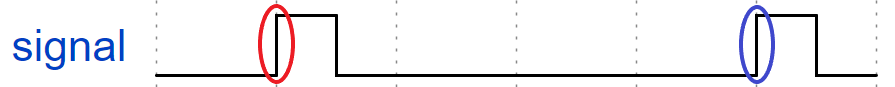
\includegraphics[width=6.1375in,height=0.59653in]{images/edge-type-01.png}
\label{fig:2}
\end{figure}

Now we can see the representation of a \emph{falling edge} configuration
for the start signal (red) and the stop signal (blue).

\hypertarget{lifetime-measurements}{%
\subsection{Lifetime measurements}\label{lifetime-measurements}}

Lifetime measurements are used to determine how long a molecule,
particle, or physical system stays in an excited state before returning
to its ground state, or to quantify the duration of a short-lived
compound. Most of these measurements are performed by measuring the time
difference between two photons.

One of the most widely used techniques for this type of measurement is
time-correlated single photon counting (TCSPC). This technique relies on
the emission of a pulse from a laser, which acts as a trigger to start
the measurement. If the laser\textquotesingle s frequency is correct, it
partially excites the sample. Subsequently, the sample decays and emits
a photon back. Some of these photons are detected by an electronic
system, which converts them into electrical pulses. These electrical
pulses mark the end of the measurement. The time difference between the
start pulse and the stop pulse is mapped onto a histogram. Ultimately,
the obtained histogram provides information about the temporal
distribution of the sample\textquotesingle s exciting state.

Tempico software is capable of capturing data in techniques that involve
the emission and detection of pulses, such as in single photon counting.
Several lifetime measurement methods can be applied depending on the
type of analysis being performed.

\hypertarget{fluorescence-lifetime-measurements}{%
\subsubsection{Fluorescence lifetime
measurements}\label{fluorescence-lifetime-measurements}}

This technique involves the use of a fluorophore to measure the time it
takes to return to the ground state from the excited state. It is
primarily used for the analysis of chemical and biological samples. The
analysis is conducted by creating an environment with a fluorophore, and
any change in the sample causes a modification in the fluorescent
environment. In this way, temporal differences associated with
interactions or changes in the sample can be obtained.

\hypertarget{description}{%
\section{Description}\label{description}}

Tempico Software is designed to facilitate the use of the Tausand
Tempico TP1004 and TP1204 devices. It is a graphical interface that
allows for time histogram measurements and \emph{lifetime} measurements.
From the software, it is possible to configure the device, as well as
save the measurement data and generated graphs in various text and image
formats, respectively. Additionally, Tempico Software provides extra
functions, such as creating custom adjustments for certain graphs, and
allowing monitoring the device to ensure the measurement is being
performed correctly.

\hypertarget{specifications}{%
\section{Specifications}\label{specifications}}

Tempico software is designed to run on devices with low requirements,
allowing any laboratory to use it. The minimum requirements for Tempico
Software to function are as follows:

\begin{itemize}
\item
  \textbf{OS}: Windows 7 Home Premium, Windows 7 Professional, Windows 7
  Ultimate, Ubuntu 20.04, mac OS Big Sur
\item
  \textbf{CPU}: Intel Pentium Dual-Core E5200
\item
  \textbf{RAM}: 1 GB
\item
  \textbf{Storage}: 500 MB available
\end{itemize}

For measurements with large data sets or long durations (greater than 6
hours), the performance of Tempico Software may decrease. However, on
higher-performance devices, this issue is mitigated.

\hypertarget{installation}{%
\section{Installation}\label{installation}}

\hypertarget{windows}{%
\subsection{Windows}\label{windows}}

The first step is to download the software from the Tausand website:
\url{https://www.tausand.com/downloads/}. From this page, an executable
file will be downloaded, which should be run to complete the
installation by following the steps provided.

When opening the installer, it will request permission to run, to which
we should respond affirmatively. After that, a window will appear asking
us to select the installation path. We can choose the desired path; by
default, the software will be installed in the Program Files folder.

\begin{figure}[H]
\centering
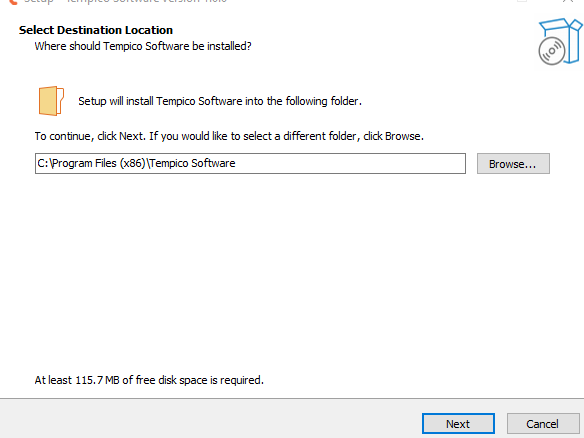
\includegraphics[width=4.2827in,height=3.21203in]{images/windows-01.png}
\label{fig:3}
\end{figure}

Next, we will be asked if we want to create a shortcut on the desktop.
To do so, we should check the corresponding box.

\begin{figure}[H]
\centering
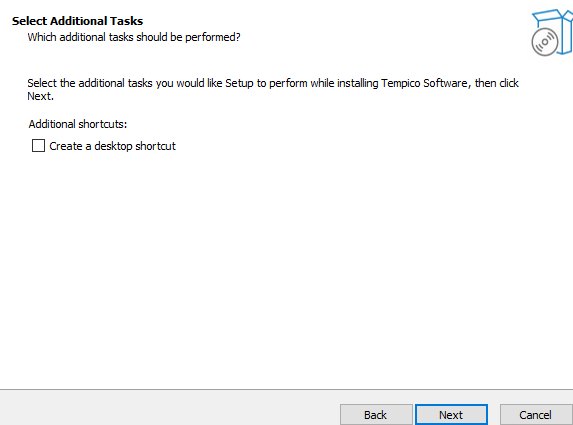
\includegraphics[width=4.76527in,height=3.53445in]{images/windows-02.png}
\label{fig:4}
\end{figure}

After completing these two steps, a tab will open showing us the
installation path, allowing us to verify it before proceeding with the
installation.

\begin{figure}[H]
\centering
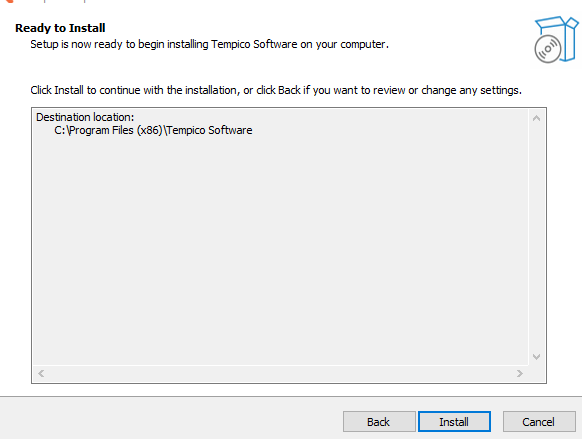
\includegraphics[width=4.18609in,height=3.15755in]{images/windows-03.png}
\label{fig:5}
\end{figure}

Once the installation process is complete, we can click "Finish". It is
important to check whether we want the program to run immediately, by
checking or unchecking the corresponding box.

\begin{figure}[H]
\centering
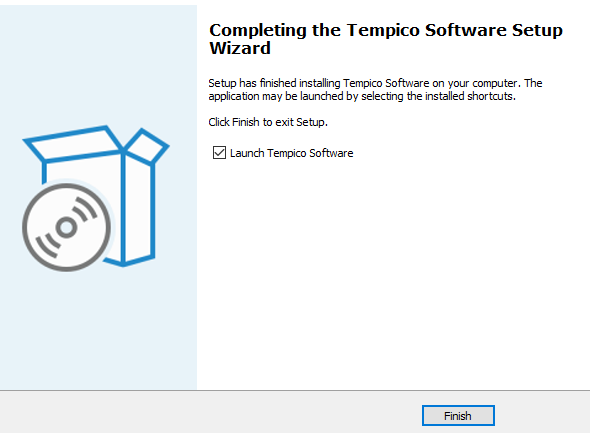
\includegraphics[width=4.68095in,height=3.43471in]{images/windows-04.png}
\label{fig:6}
\end{figure}

\hypertarget{ubuntu}{%
\subsection{Ubuntu}\label{ubuntu}}

On Ubuntu, you only need to download the compressed (.zip) file from the
official page. Once downloaded, extract its contents and run the
AppImage file found inside. With this process, Tempico Software will be
ready to use on your system.

\begin{figure}[H]
\centering
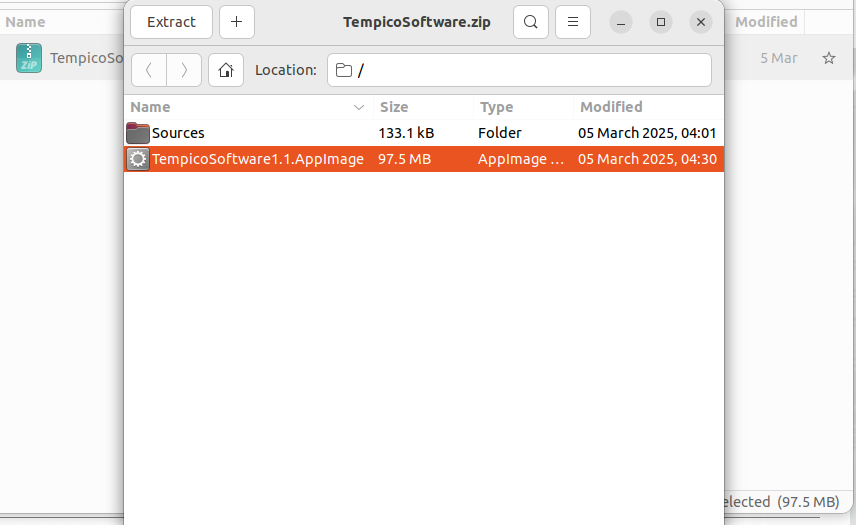
\includegraphics[width=6.1375in,height=3.76458in]{images/ubuntu-01.png}
\label{fig:7}
\end{figure}

\begin{figure}[H]
\centering
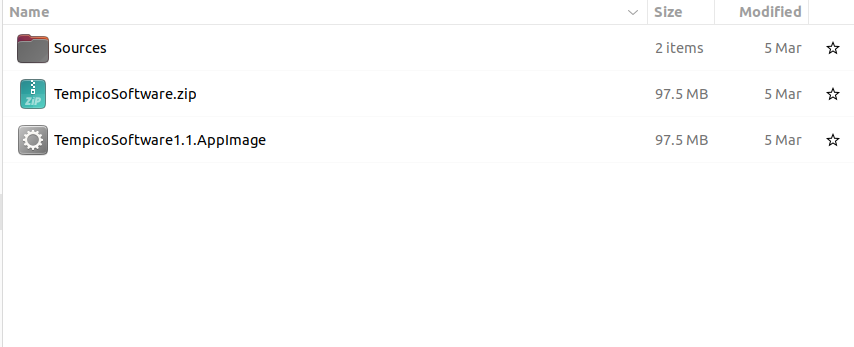
\includegraphics[width=6.1375in,height=2.49375in]{images/ubuntu-02.png}
\label{fig:8}
\end{figure}

\hypertarget{mac}{%
\subsection{Mac}\label{mac}}

On macOS, you only need to download the .zip file and extract its
contents to your preferred folder. The file named ``Tempico Software''
is the one you need to run to launch the program.

\begin{figure}[H]
\centering
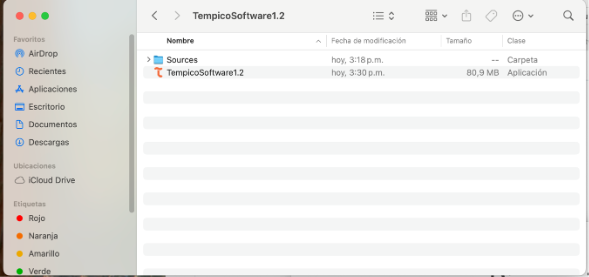
\includegraphics[width=6.13542in,height=2.88542in]{images/mac-01.png}
\label{fig:9}
\end{figure}

\hypertarget{software-operation}{%
\section{Software operation}\label{software-operation}}

The software is used in the same way across all operating systems;
however, the preparations for running the software may differ depending
on the operating system.

\hypertarget{system-configuration}{%
\subsection{System configuration}\label{system-configuration}}

To ensure the proper functioning of Tempico Software, it is necessary to
perform certain validations on the operating system.

\hypertarget{windows-1}{%
\subsubsection{Windows}\label{windows-1}}

You should ensure that the Tempico device is recognized by the COM
ports. To do this, follow these steps: If, when connecting and turning
on the device for the first time, a window appears indicating that the
Tempico device is being configured, it means that Windows has recognized
it correctly. If this does not happen, you can access the Device Manager
without having the device connected and navigate it to the COM and LPT
ports section. Then, connect and turn on the device. The port table
should be updated; if it does not, close and reopen the window. When
doing so, a new COM device should appear, indicating that the Tempico
has been correctly detected.

\hypertarget{ubuntu-1}{%
\subsubsection{Ubuntu}\label{ubuntu-1}}
\begin{center}
    \textbf{ls /dev/tty*}
\end{center}

In this case, it is also necessary to verify that the ports are
correctly detecting the device. To do this, we will use the command
above, which lists the devices connected to the serial ports. First, we
will run this command without the Tempico device connected and then run
it again with the device connected. We will observe which new device has
been detected

\begin{center}
    \textbf{sudo adduser "username" dialout}
\end{center}


If an error occurs indicating that the serial port could not be opened,
it is possible that the user does not belong to the dialout group. To
resolve this, we will execute the command above. This will allow us to
access the system\textquotesingle s serial ports.

Si el comando no es suficiente y el software sigue lanzando errores debe
verificarse cual es el puerto tty que se esta usando y debe ejecutarse
lo siguiente:

\begin{center}
    \textbf{sudo chmod 666 /dev/tty"port"}
\end{center}

\hypertarget{mac-1}{%
\subsubsection{Mac}\label{mac-1}}

\begin{center}
    \textbf{ls /dev/tty.*}
\end{center}


To verify that the device is correctly connected to Mac, we must, with
the Tempico turned off, execute the command above. This will provide a
list of connected devices. Then, we run the command again with the
Tempico turned on and observe which new port appears in the list.

If the device is not detected, the software will not recognize the
connection, making it impossible to use the software. In this case,
please contact Tausand support at: support@tausand.com.

\hypertarget{open-the-software-and-select-a-tempico-device}{%
\subsection{Open the software and select a Tempico
device}\label{open-the-software-and-select-a-tempico-device}}

When opening the software, an image with the program\textquotesingle s
logo is displayed, followed by a window that allows you to select the
device with the port to which you want to connect the device.

\begin{figure}[H]
\centering

\includegraphics[width=3.29565in,height=1.47555in]{images/open-the-software-and-select-a-tempico-01.png}
\label{fig:10}
\end{figure}

\begin{figure}[H]
\centering
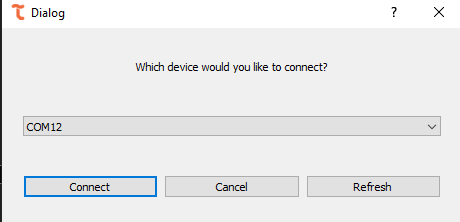
\includegraphics[width=4.79234in,height=2.31282in]{images/open-the-software-and-select-a-tempico-02.png}
\label{fig:11}
\end{figure}

If the software is opened and the device is not turned on, the window
will not recognize the connection. Therefore, it is necessary to click
the "Refresh" button to update the list of ports with a Tempico device.

Once connected, the software will open with all options enabled for use.
The software always opens in the histogram window.

\begin{figure}[H]
\centering
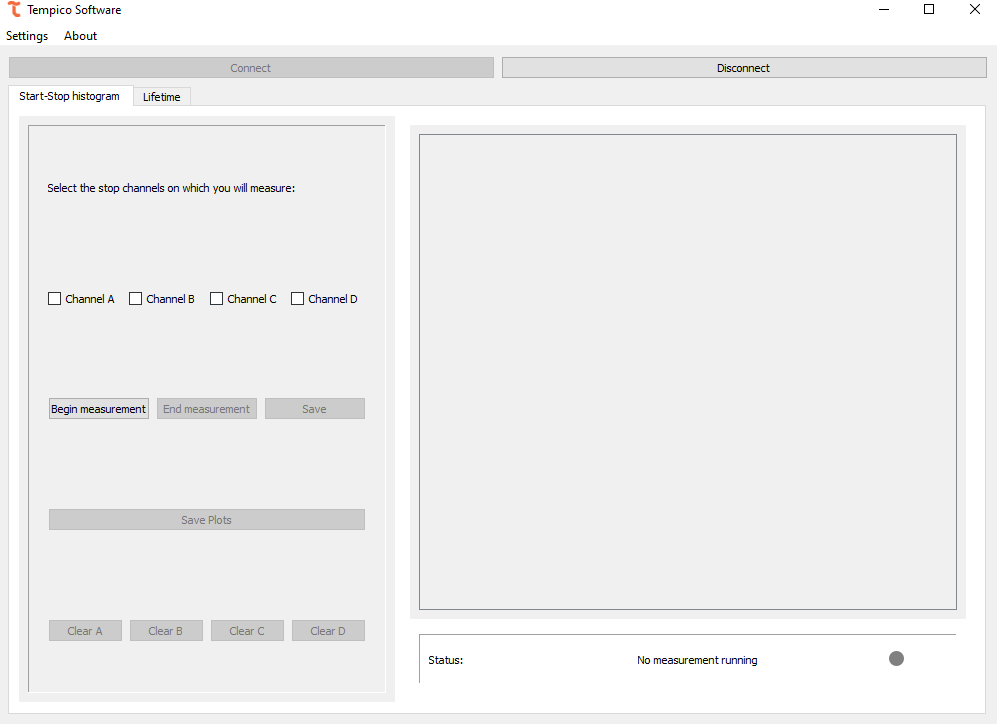
\includegraphics[width=5.42142in,height=3.93694in]{images/open-the-software-and-select-a-tempico-03.png}
\label{fig:12}
\end{figure}

If "Cancel" is selected or the dialog box is closed, the options to
select a channel or start a measurement will not be available.

\begin{figure}[H]
\centering
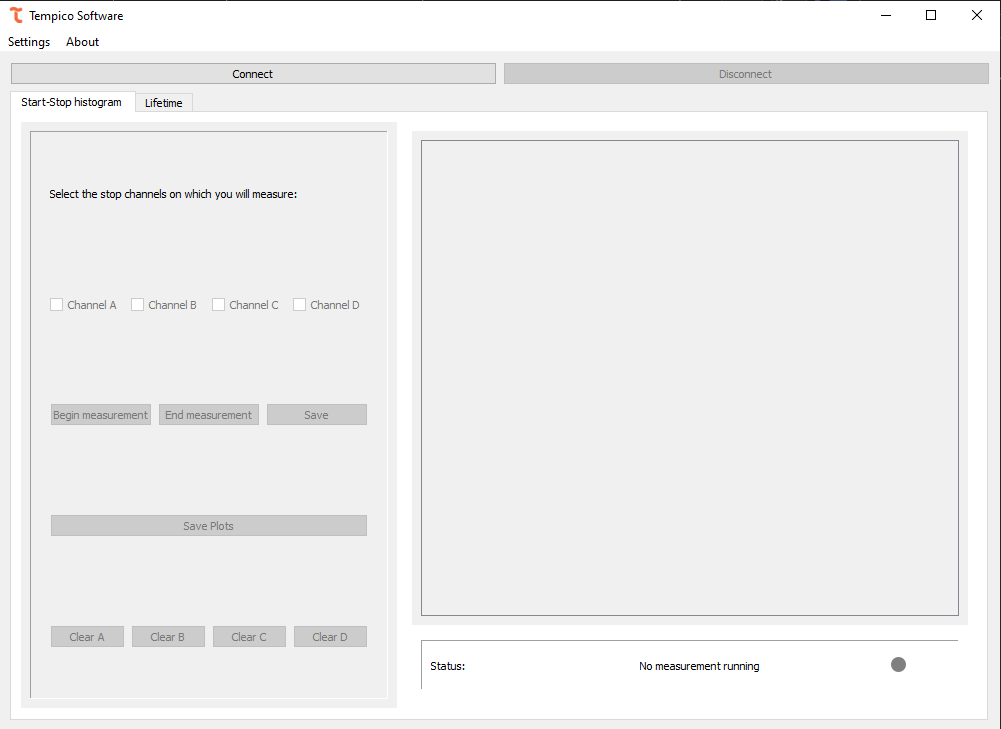
\includegraphics[width=5.35801in,height=3.90181in]{images/open-the-software-and-select-a-tempico-04.png}
\label{fig:13}
\end{figure}

If this happens, we can click the "Connect" button again to search for
devices.

\begin{figure}[H]
\centering
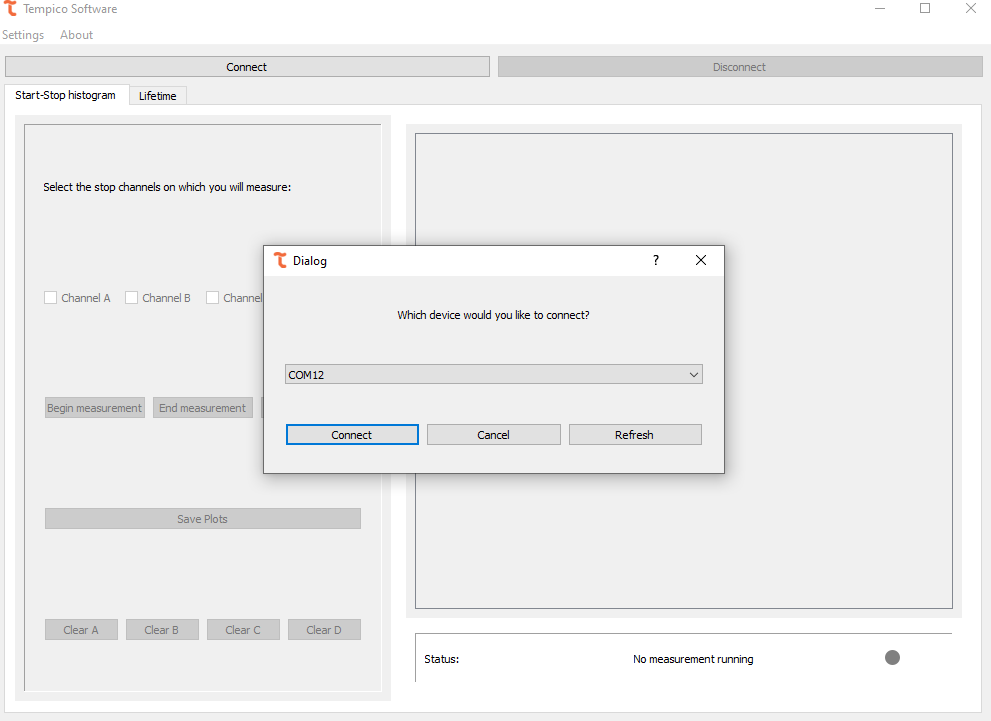
\includegraphics[width=5.3761in,height=3.91132in]{images/open-the-software-and-select-a-tempico-05.png}
\label{fig:14}
\end{figure}

It is also possible to disconnect the device if we want to use another
Tempico. To do so, click the "Disconnect" button. If an error occurs
while connecting to the device, the following error window will be
displayed:

\begin{figure}[H]
\centering
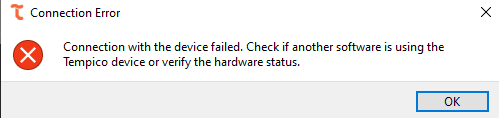
\includegraphics[width=5.19864in,height=1.22934in]{images/open-the-software-and-select-a-tempico-06.png}
\label{fig:15}
\end{figure}

If this happens, it should be verified that no other program has
established communication with the Tempico, and ensure that the USB
connection, whether the cable or the physical port, is in good
condition. If no issues are found after verifying this, support should
be contacted to find a solution to the problem.

\hypertarget{channel-settings}{%
\subsection{Channel settings}\label{channel-settings}}

Once the connection with the device is established, it is possible to
access the settings for each channel. To do so, go to the tab at the
top, select "Settings," and then choose "Channel Settings," where you
can view the current settings of the device:

\begin{figure}[H]
\centering
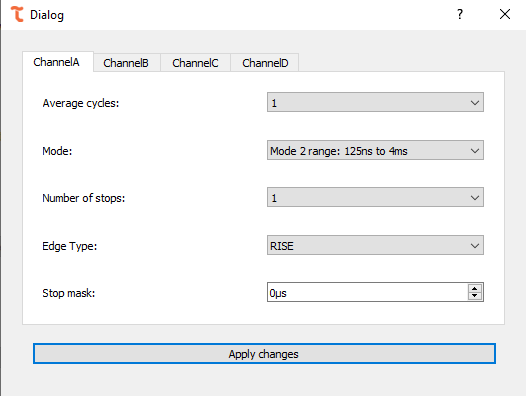
\includegraphics[width=5.47993in,height=4.12558in]{images/channel-settings-01.png}
\label{fig:16}
\end{figure}

For each channel, you can modify the number of average cycles, the mode
that defines the time range for measurements, the number of stops, the
edge type and the stop mask. All these options provide a dropdown menu
with the options allowed by the device (refer to the Tausand Tempico
manual for more information), except for the stop mask.

\begin{figure}[H]
\centering
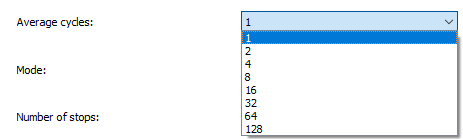
\includegraphics[width=4.82359in,height=1.44812in]{images/channel-settings-02.png}
\label{fig:17}
\end{figure}

\begin{figure}[H]
\centering
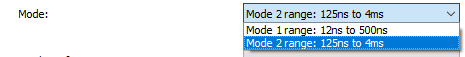
\includegraphics[width=4.84443in,height=0.59383in]{images/channel-settings-03.png}
\label{fig:18}
\end{figure}

\begin{figure}[H]
\centering
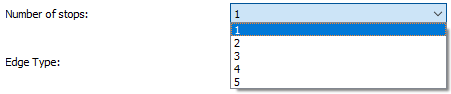
\includegraphics[width=4.69857in,height=0.9793in]{images/channel-settings-04.png}
\label{fig:19}
\end{figure}

\begin{figure}[H]
\centering
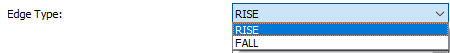
\includegraphics[width=4.68815in,height=0.55216in]{images/channel-settings-05.png}
\label{fig:20}
\end{figure}

For the "Stop Mask," you can enter a number between 0 and 4000 $\mu$s.

\begin{figure}[H]
\centering
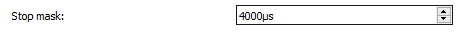
\includegraphics[width=4.82359in,height=0.37505in]{images/channel-settings-06.png}
\label{fig:21}
\end{figure}

Once the desired values have been changed, click the "Apply Changes"
button to transmit the changes to the device. To verify the changes, you
can return to the tab and check that the values are the same as those
previously set.

\hypertarget{general-settings}{%
\subsection{General settings}\label{general-settings}}

The software features another window that displays the options affecting
all channels of the device, including the start channel. To access it,
go to the top, select "Settings," and then click on "General Settings":

\begin{figure}[H]
\centering
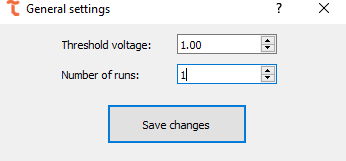
\includegraphics[width=3.60467in,height=1.67732in]{images/general-settings-01.png}
\label{fig:22}
\end{figure}

From there, it is possible to set the "Threshold Voltage" and the
"Number of Runs" for the measurements. The "Threshold Voltage" value
allows a range between 0.90 and 1.60, with increments of 0.01, while the
"Number of Runs" allows up to a value of 1000 (for more information on
these settings, refer to the device manual). Once the changes have been
made, click on "Save Changes," and to confirm, return to the tab and
check that the values are the same as those set.

\hypertarget{tp1200-settings}{%
\subsection{TP1200 settings}\label{tp1200-settings}}

The TP1200 versions from Tempico are equipped with an internal periodic
pulse generator, which can be configured through the Tempico Software.
To perform this configuration, the user must access the settings menu
and select the Signal Generator option. In this section, it is possible
to define whether the signals acquired by each channel originate from an
external source, meaning a direct electrical connection to the device,
by selecting ``External'', or whether the signals originate from the
internal pulse generator by selecting ``Internal''.

Below the signal source selection for each channel, the pulse frequency
of the internal generator can be adjusted. The available frequency range
spans from 10 Hz to 9,450,000 Hz.

\begin{figure}[H]
\centering
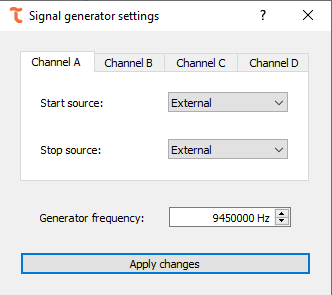
\includegraphics[width=3.45882in,height=3.07335in]{images/tp1200-settings-01.png}
\label{fig:23}
\end{figure}

\hypertarget{file-path-settings}{%
\subsection{File path settings}\label{file-path-settings}}

In this dialog window, it is possible to modify the path where the data
is stored, as well as the prefixes used to save the files from each tab.
Each file is saved with the defined prefix followed by the date it was
generated, ensuring an organized and easily traceable naming scheme.
Within this window, three options are available: Apply
Changes(
\includegraphics[width=1.14202in,height=0.13577in]{images/file-path-settings-01.png}),
which updates the configuration according to the entered values;
Cancel(
\includegraphics[width=0.9903in,height=0.14645in]{images/file-path-settings-02.png}),
which closes the window without applying any changes; and Default
Settings(
\includegraphics[width=1.14724in,height=0.14646in]{images/file-path-settings-03.png}),
which restores the default values. It is important to note that this
last option will not take effect immediately, since the values will only
be applied once the user presses apply changes again.

\begin{figure}[H]
\centering
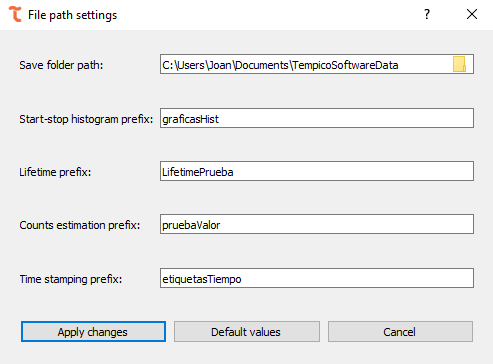
\includegraphics[width=3.99841in,height=2.95218in]{images/file-path-settings-04.png}
\label{fig:24}
\end{figure}

\hypertarget{start-stop-histogram-measurements}{%
\subsection{Start-stop histogram
measurements}\label{start-stop-histogram-measurements}}

"Start-stop" measurements are those that capture data from the basic
functionality of the Tempico device. When a start pulse is received and,
subsequently, a stop pulse arrives, the temporal difference between the
two pulses is obtained. This point is plotted on a frequency histogram.

\hypertarget{perform-a-measurement}{%
\subsubsection{Perform a measurement}\label{perform-a-measurement}}

To start the "start-stop" measurements, the channels to be sampled must
be selected. To do so, check the corresponding checkboxes located on the
left side of the window.

\begin{figure}[H]
\centering
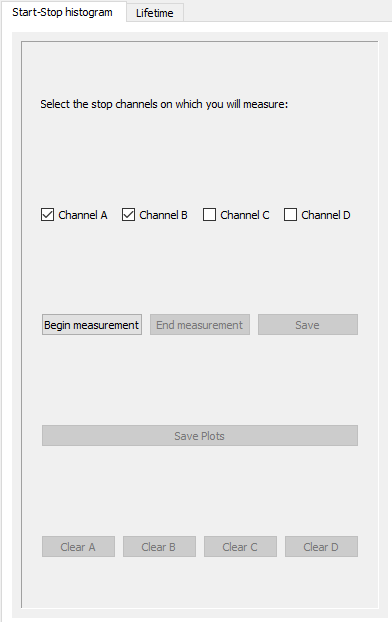
\includegraphics[width=2.67985in,height=4.25221in]{images/perform-a-measurement-01.png}
\label{fig:25}
\end{figure}

Afterward, click on "Begin Measurement"
(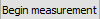
\includegraphics[width=0.73867in,height=0.14035in]{images/perform-a-measurement-02.png}).
Depending on the number of channels selected, the corresponding graphs
will be created on the right side of the window. Once the measurement
begins, a histogram will be obtained for each channel.

\begin{figure}[H]
\centering
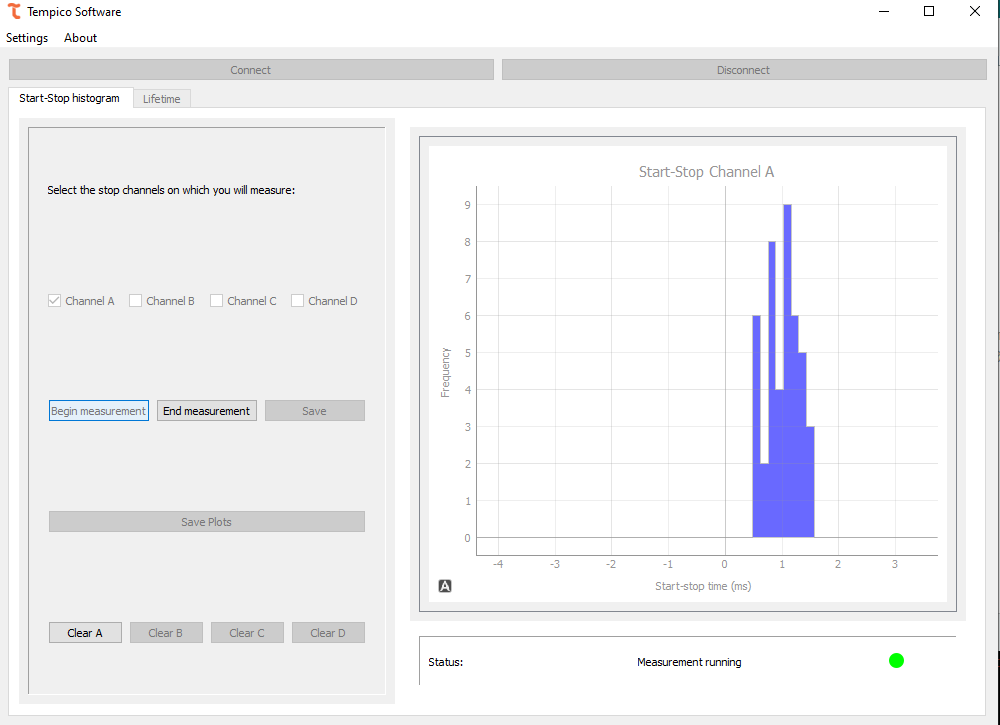
\includegraphics[width=6.1375in,height=4.44931in]{images/perform-a-measurement-03.png}
\label{fig:26}
\end{figure}

It is possible to interact with the graphs generated for each channel,
either by dragging the range or adjusting the zoom with the mouse wheel.
The histogram is generated according to the zoom level of the plot.
Therefore, by zooming in and examining the range in more detail, more
precise points will be obtained, indicating where each data point falls.

\begin{figure}[H]
\centering
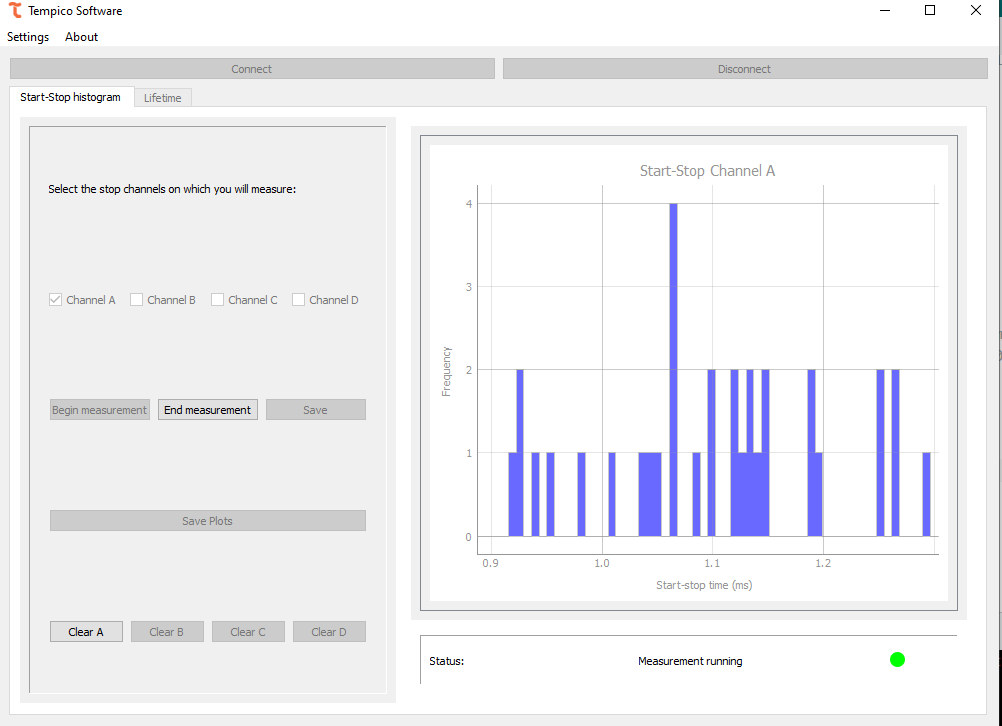
\includegraphics[width=3.4363in,height=2.9099in]{images/perform-a-measurement-04.png}
\label{fig:27}
\end{figure}

Conversely, if we increase the temporal axis range, the number of bars
will decrease.

\begin{figure}[H]
\centering
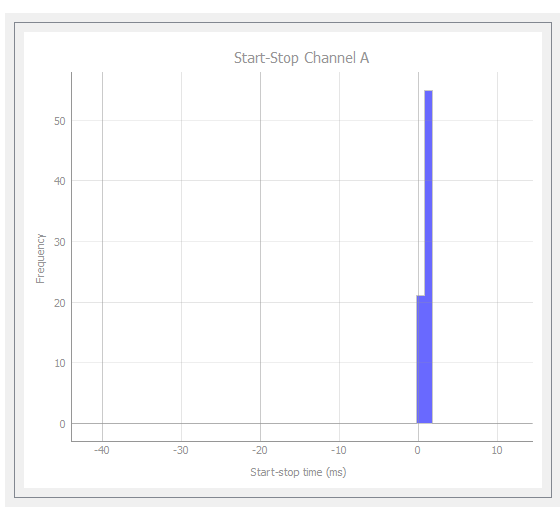
\includegraphics[width=3.70537in,height=3.36792in]{images/perform-a-measurement-05.png}
\label{fig:28}
\end{figure}

Right-clicking on the graph enables additional options for interacting
with it, such as manual zoom on each axis, changing the selection mode
with the mouse, or exporting the image. Since these options come from
the library used to generate the graph, it is not recommended to
interact with the graph through these functions. However, the user is
free to use them if desired.

\begin{figure}[H]
\centering
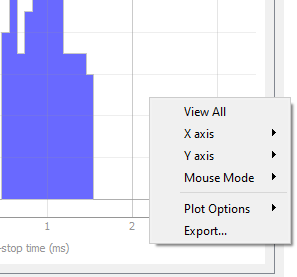
\includegraphics[width=2.86059in,height=2.66796in]{images/perform-a-measurement-06.png}
\label{fig:29}
\end{figure}

The status bar indicates whether the measurement is being carried out
correctly. If any channel is not receiving data, the status bar will
display a message to indicate this.

\begin{figure}[H]
\centering
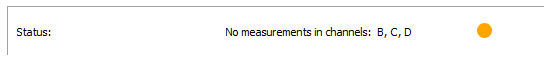
\includegraphics[width=5.17045in,height=0.69064in]{images/perform-a-measurement-07.png}
\label{fig:30}
\end{figure}

If the start channel is not receiving data, the following message will
be displayed:

\begin{figure}[H]
\centering
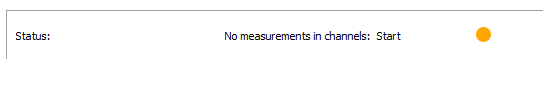
\includegraphics[width=4.93412in,height=0.75978in]{images/perform-a-measurement-08.png}
\label{fig:31}
\end{figure}

A possible solution to this issue is configuring the threshold voltage.
It is recommended to set it to 1.6 V and check if the measurement is
performed correctly. If the error persists, try different values for
this parameter. If the issue continues and it is determined that it is
not a fault in the setup or the input signal, Tausand support should be
contacted.

Start-stop histograms are designed to take measurements indefinitely.
Once the experiment is considered complete, click the "End Measurement"
button (
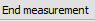
\includegraphics[width=0.63729in,height=0.14087in]{images/perform-a-measurement-09.png})
to stop data collection. If you wish to clear the data during the
experiment, there\textquotesingle s no need to stop the measurement. At
the bottom of the left menu, there are "Clear" buttons to erase both the
data and current graphs. Four buttons are available to clear data for
each channel independently (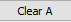
\includegraphics[width=0.52823in,height=0.16368in]{images/perform-a-measurement-10.png},

\includegraphics[width=0.61629in,height=0.1697in]{images/perform-a-measurement-11.png},

\includegraphics[width=0.6656in,height=0.17812in]{images/perform-a-measurement-12.png},
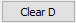
\includegraphics[width=0.65672in,height=0.19874in]{images/perform-a-measurement-13.png}).

For Tempico TP1200 versions, this window can measure negative ranges
down to --200 ns. The purpose of this capability is to allow more
accurate measurements of values close to zero, which in the TP1000
version are limited by its technical specifications.

\begin{figure}[H]
\centering
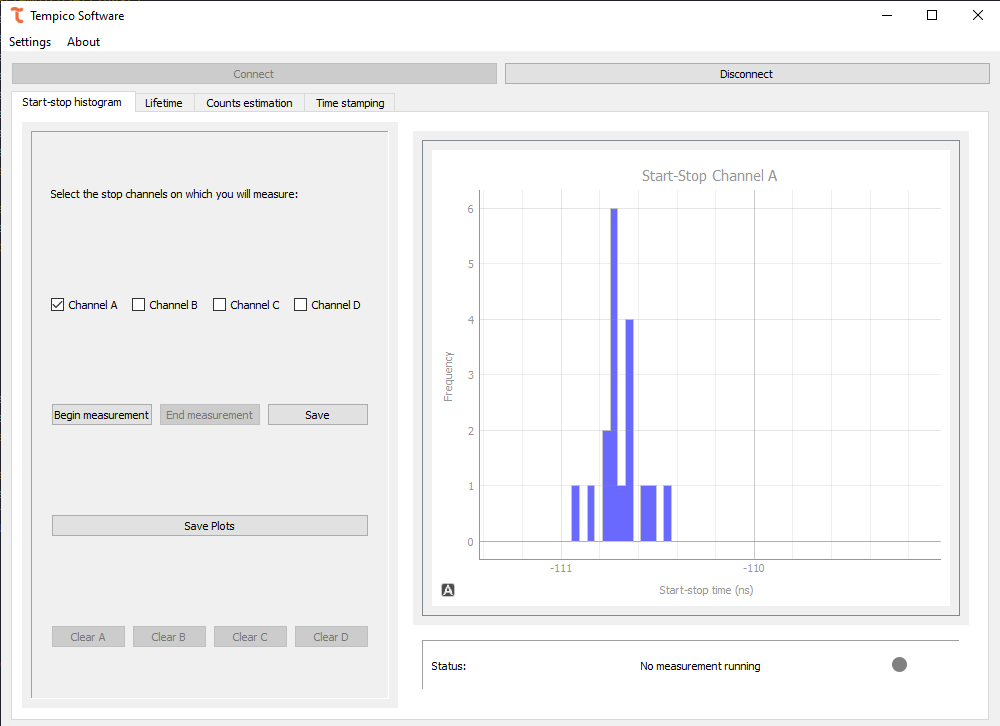
\includegraphics[width=6.1375in,height=4.45556in]{images/perform-a-measurement-14.png}
\label{fig:33}
\end{figure}

\hypertarget{save-data-and-plots}{%
\subsubsection{Save data and plots}\label{save-data-and-plots}}

If the user wishes to save the graphed data, they should click the save
button
(
\includegraphics[width=0.69876in,height=0.16072in]{images/save-data-and-plots-01.png}
), which will open a menu allowing them to select the format in which to
save the files.

\begin{figure}[H]
\centering
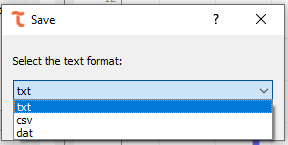
\includegraphics[width=3.00042in,height=1.51063in]{images/save-data-and-plots-02.png}
\label{fig:34}
\end{figure}

After selecting the desired format, click the accept button (
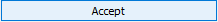
\includegraphics[width=1.09749in,height=0.11076in]{images/save-data-and-plots-03.png}),
which will display a dialog box indicating that the file has been saved
successfully

\begin{figure}[H]
\centering
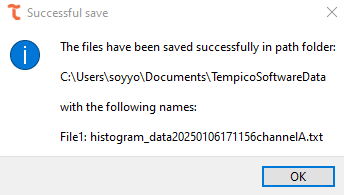
\includegraphics[width=2.3672in,height=1.34187in]{images/save-data-and-plots-04.png}
\label{fig:35}
\end{figure}

Files are saved in all operating systems in the "TempicoSoftwareData"
folder within "Documents." By default, this folder is automatically
created when the program is opened for the first time.

The data is saved in the same format. First, it includes the
configuration applied when the data was collected, followed by the raw
histogram information. This allows the user, if desired, to later
manipulate the data according to their needs.

\begin{figure}[H]
\centering
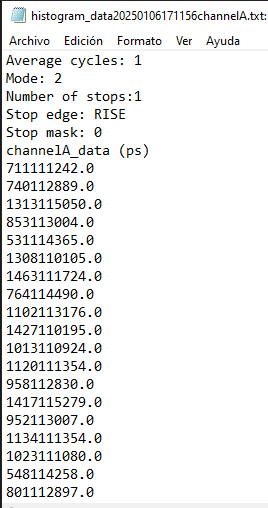
\includegraphics[width=2.0407in,height=3.8682in]{images/save-data-and-plots-05.png}
\label{fig:36}
\end{figure}

If the user wishes to save the graphs generated by the software during
the measurement, they must click on the "Save Plots" button
(
\includegraphics[width=2.23435in,height=0.14943in]{images/save-data-and-plots-06.png}
). A window will then open, allowing them to select the image format.

\begin{figure}[H]
\centering
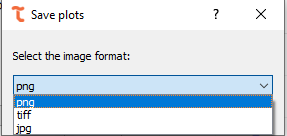
\includegraphics[width=2.99in,height=1.41686in]{images/save-data-and-plots-07.png}
\label{fig:37}
\end{figure}

After selecting the format, click the "Accept" button (
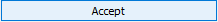
\includegraphics[width=1.09749in,height=0.11076in]{images/save-data-and-plots-03.png}).
As with the previous case, a dialog box will appear indicating that the
image has been successfully saved. The image will be saved in the same
location as the text files, across all operating systems.

\begin{figure}[H]
\centering
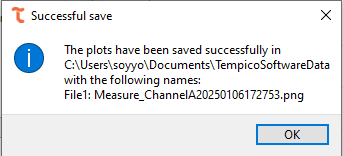
\includegraphics[width=3.57342in,height=1.62523in]{images/save-data-and-plots-08.png}
\label{fig:38}
\end{figure}

The saved image is the one displayed in the software at the moment of
clicking "Accept." Therefore, the zoom applied to the graph will also be
reflected when saving the image. If multiple channels are selected for
measurement, the 4 images will be saved separately.

\begin{figure}[H]
\centering
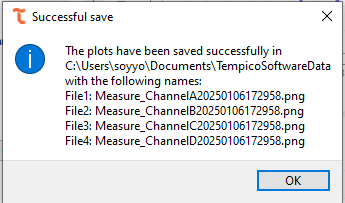
\includegraphics[width=3.59425in,height=2.11488in]{images/save-data-and-plots-09.png}
\label{fig:39}
\end{figure}

\hypertarget{lifetime-histograms}{%
\subsection{Lifetime histograms}\label{lifetime-histograms}}

To record lifetime measurements based on the time difference between
input pulses and emitted excitation pulses, Tempico Software provides
multiple tools to fulfill this functionality.

\hypertarget{settings-before-a-measurement}{%
\subsubsection{Settings before a
measurement}\label{settings-before-a-measurement}}

Unlike the measurement of start and stop histograms, the preliminary
setup for a lifetime measurement is a bit more elaborate. First, we must
select the start channel and the stop channel for our measurements.

If a channel other than start is selected to initiate the measurement, a
periodic electrical signal must be added to the start channel, as
Tempico cannot measure signals on stop channels without a registered
start event. This configuration risks losing data that arrives before
the periodic signal is emitted. The pulse period must be short enough to
reduce data loss. Tempico does not register stops occurring within less
than 12 ns, making this setup useful for mitigating such effects.

After selecting the channel, the bin width must be chosen, representing
the histogram\textquotesingle s bar width. For example, with a bin width
of 12 ns, if there are two measurements at 1 ns and 5 ns, both will
contribute to the same histogram bar\textquotesingle s frequency. The
number of bins prevents histogram saturation and usually limits the time
axis range. For instance, selecting a bin width of 480 ps and 50 bins
results in a 24 ns range. Unlike start-stop histograms, lifetime
measurements are designed with a limit, allowing the number of
measurements to be specified. A measurement is counted when both start
and stop channels record a value.

\begin{figure}[H]
\centering
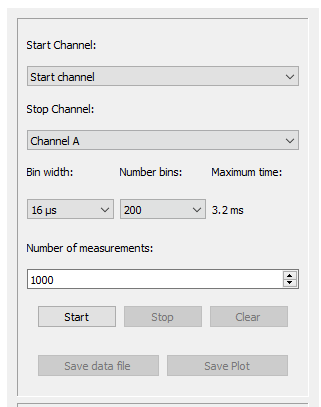
\includegraphics[width=3.09395in,height=3.92285in]{images/settings-before-a-measurement-01.png}
\label{fig:40}
\end{figure}

It\textquotesingle s important to clarify that the configurations for
the number of runs, number of stops, stop mask, and mode have no effect
on this measurement. By default, the program sets the number of runs to
100, the number of stops to 1, the stop mask to 0, and the mode
according to the maximum time parameter. If the maximum time exceeds 500
ns, the measurement operates in mode 2; otherwise, it operates in mode
1.

\hypertarget{perform-a-measurement-1}{%
\subsubsection{Perform a measurement}\label{perform-a-measurement-1}}

Once the desired configuration is selected, click the start button (
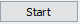
\includegraphics[width=0.46116in,height=0.13835in]{images/perform-a-measurement-1-01.png})
to begin the measurement. Like start-stop histograms, the program
displays a status bar indicating the measurement\textquotesingle s
progress. If any channel is not recording, it will be shown. In this
case, the percentage of the measurement is also displayed, as the number
of desired measurements can be specified.

\begin{figure}[H]
\centering
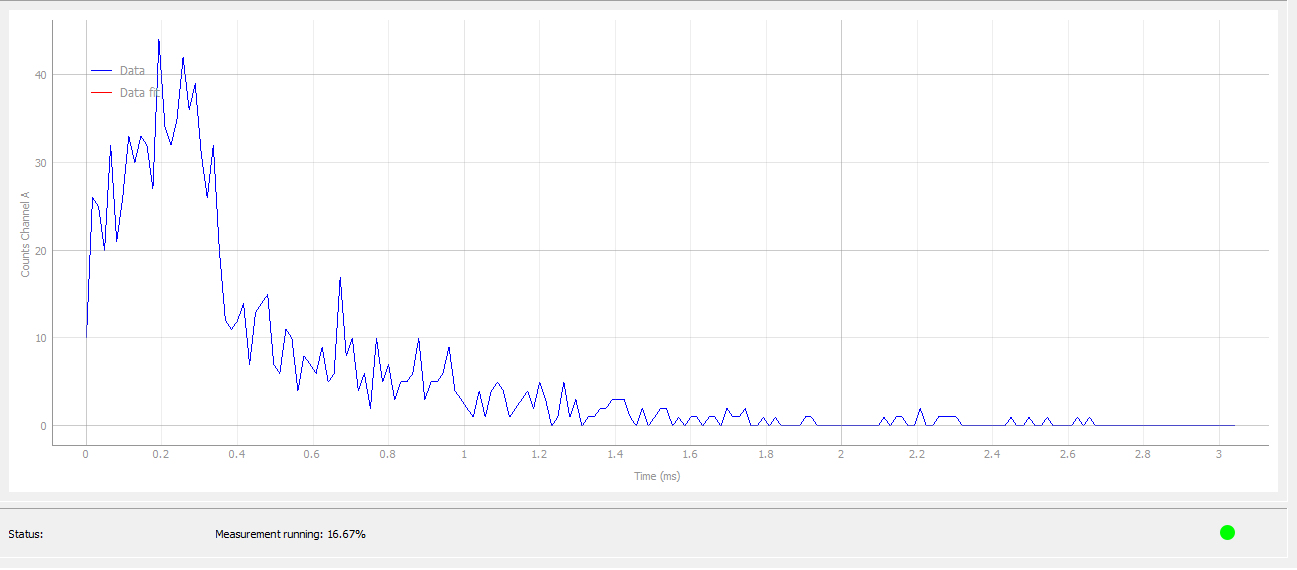
\includegraphics[width=6.1375in,height=2.69722in]{images/perform-a-measurement-1-02.png}
\label{fig:41}
\end{figure}

\begin{figure}[H]
\centering
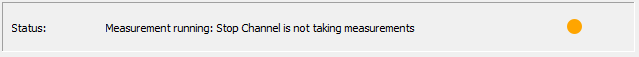
\includegraphics[width=6.1375in,height=0.54722in]{images/perform-a-measurement-1-03.png}
\label{fig:42}
\end{figure}

The program also provides additional information about the measurement
status, including the total number of starts, the total number of
complete measurements (i.e., start and stop), and the total elapsed time
in HH:MM:SS format.

\begin{figure}[H]
\centering
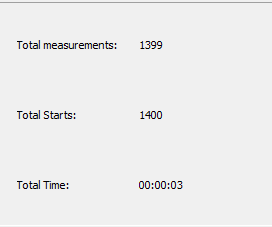
\includegraphics[width=2.83373in,height=2.36491in]{images/perform-a-measurement-1-04.png}
\label{fig:43}
\end{figure}

\hypertarget{fitting}{%
\subsubsection{Fitting}\label{fitting}}

Con el fin de obtener más información acerca de una medición, el usuario
puede realizar un fit sobre la gráfica. Al realizar el fit obtiene en la
tabla de la esquina superior derecha información más detallada acerca de
los parametros de la ecuación a ajustar. Obtiene sus valores, su
desviación estándar y sus respectivas unidades.

\begin{figure}[H]
\centering
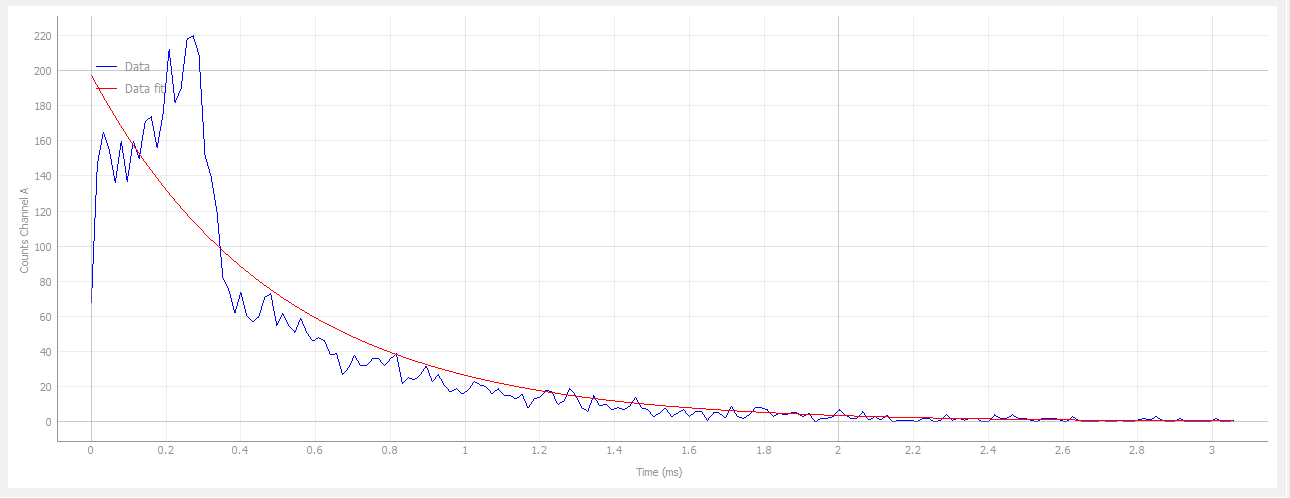
\includegraphics[width=6.1375in,height=2.36944in]{images/fitting-01.png}
\label{fig:44}
\end{figure}

\begin{figure}[H]
\centering
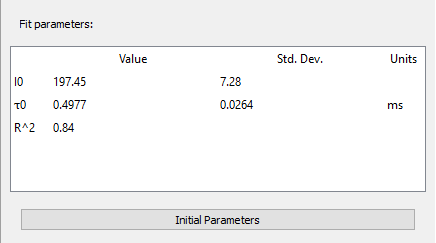
\includegraphics[width=4.5423in,height=2.5316in]{images/fitting-02.png}
\label{fig:45}
\end{figure}

In some cases, reliable values may not be estimated, and the adjustment
will indicate "nan" for those parameters. The quality of the fitness
depends on the initial parameters set before the estimation. Therefore,
users are free to modify these parameters. They can also revert to the
default values provided by the software.

\begin{figure}[H]
\centering
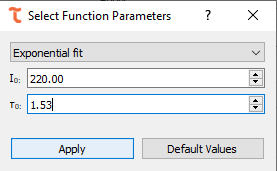
\includegraphics[width=2.88582in,height=1.7815in]{images/fitting-03.png}
\label{fig:46}
\end{figure}

The software offers various types of adjustments:

\hypertarget{exponential}{%
\paragraph{Exponential}\label{exponential}}

\[I_{0}e^{\frac{- \tau}{\tau_{0}}}\]

For fluorescence decay processes and certain radioactive processes, it
is common to encounter exponential distribution. This distribution
involves two parameters: by default, the initial value of
\(I_{0}\)\hspace{0pt} is set to the maximum found on the graph, and
\(\tau_{0}\)\hspace{0pt} corresponds to the average of the measured
times.

\hypertarget{shifted-exponential}{%
\paragraph{Shifted exponential}\label{shifted-exponential}}

\[I_{0}e^{\frac{- \tau + \alpha}{\tau_{0}}} + b\]

In some cases, an exponential distribution may exhibit a shift due to
noise or inherent system characteristics. For these situations, an
option for an exponential distribution with a shift is provided,
allowing the user to correct the shift and obtain a pure exponential
distribution. The initial parameters \(I_{0}\)\hspace{0pt} and
\(\tau_{0}\)\hspace{0pt} are the same as those used by default in the
exponential distribution. However, the additional parameters
\(\alpha\ \)and \(b\) are set to 0 by default.

\hypertarget{kohlrausch}{%
\paragraph{Kohlrausch}\label{kohlrausch}}

\[I_{0}e^{\left( \frac{- \tau\ \ }{\tau_{0}} \right)^{\beta\ }}\]

In the case of fluorescence lifetime measurements, interactions may
occur both in the environment and with the fluorescent material, which
can be interpreted as noise in the final measurement. To obtain a
profile that represents the dynamics of fluorescence, a Kohlrausch fit
can be used. The default initial value for the \(\beta\) parameter is 1.

\hypertarget{double-exponential}{%
\paragraph{Double exponential}\label{double-exponential}}

\[I_{0}\left( \alpha\ e^{\frac{- \tau}{\tau_{0}\ }} + (1 - \alpha)e^{\frac{- \tau}{\tau_{1}\ }} \right)\]

In some cases, the data may have more than one component, and the user
may wish to separate the parameters of each. For these cases, a double
exponential fit can be used. The default values are the same as those
used in the exponential distribution; the default value for \(\alpha\)
is 1, and the value for \(\tau_{1}\)is the same as \(\tau_{0}\).

\hypertarget{save-data-and-plots-1}{%
\subsubsection{Save data and plots}\label{save-data-and-plots-1}}

Like the histogram functionality, the user has the option to save both
the data and the image. If the user clicks the \textbf{Save Data File}
button (

\includegraphics[width=0.71357in,height=0.13379in]{images/save-data-and-plots-1-01.png}),
a window will appear to select the desired format for saving the data.
The user can choose between txt, csv, or dat formats.

\begin{figure}[H]
\centering
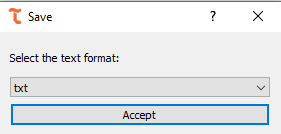
\includegraphics[width=2.92749in,height=1.36994in]{images/save-data-and-plots-1-02.png}
\label{fig:47}
\end{figure}

If the user clicks the \textbf{Accept} button
(
\includegraphics[width=1.5837in,height=0.1361in]{images/save-data-and-plots-1-03.png}
), a window will appear confirming that the file has been successfully
saved and displaying the path where it was stored.

\begin{figure}[H]
\centering
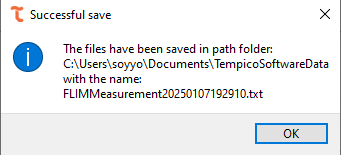
\includegraphics[width=3.55258in,height=1.61481in]{images/save-data-and-plots-1-04.png}
\label{fig:48}
\end{figure}

If the user clicks \textbf{Save Plot}
(
\includegraphics[width=0.70305in,height=0.13545in]{images/save-data-and-plots-1-05.png}
), they can choose from three formats: PNG, TIFF, and JPG. Upon clicking
the \textbf{Accept} button, a window will confirm that the file has been
successfully saved and display the path where it was stored.

\begin{figure}[H]
\centering
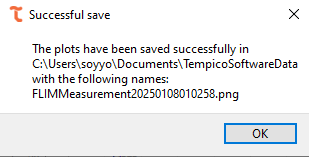
\includegraphics[width=3.2192in,height=1.63565in]{images/save-data-and-plots-1-06.png}
\label{fig:49}
\end{figure}

If an adjustment is applied, both the image and the text data will
include the equation of the adjustment made, along with the calculated
parameters.

\begin{figure}[H]
\centering
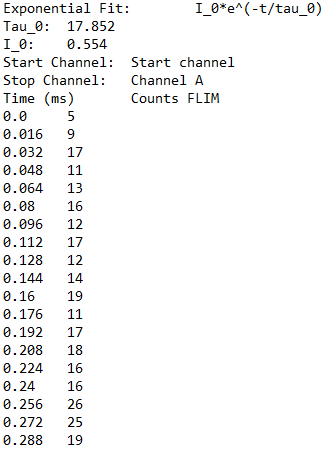
\includegraphics[width=2.70434in,height=3.69073in]{images/save-data-and-plots-1-07.png}
\label{fig:50}
\end{figure}

\begin{figure}[H]
\centering
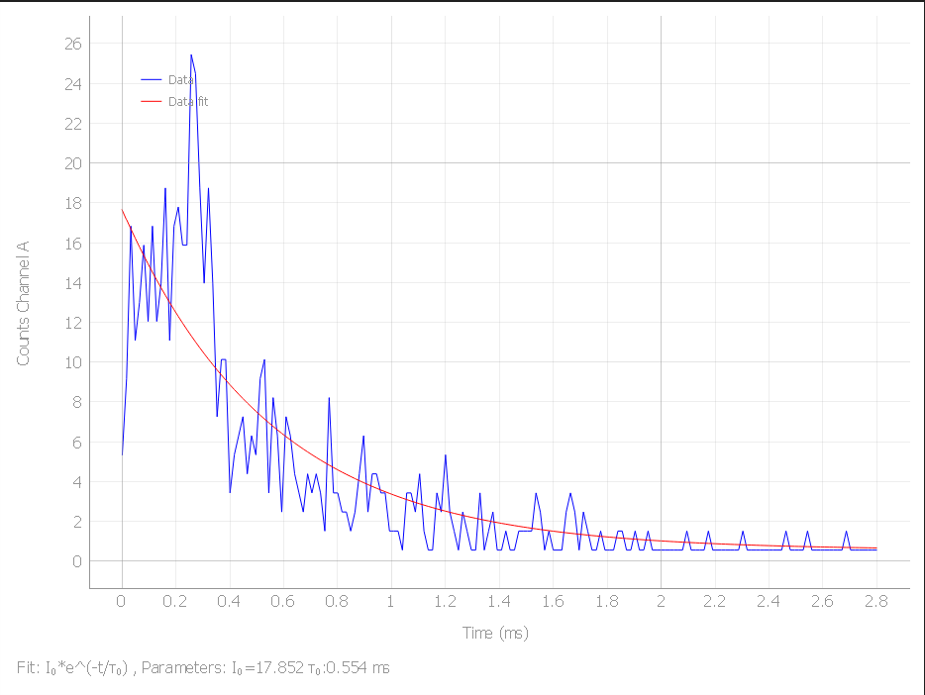
\includegraphics[width=5.33219in,height=4.00669in]{images/save-data-and-plots-1-08.png}
\label{fig:51}
\end{figure}

\hypertarget{counts-estimation}{%
\subsection{Counts estimation}\label{counts-estimation}}

Tempico Software does not directly provide the exact count of pulses
received on each channel, since the Tempico device accepts a maximum of
five incoming pulses after a start pulse. However, the software offers a
feature that enables reliable count estimation by analyzing the time
intervals between pulses.

\hypertarget{settings-for-signal-measurement}{%
\subsubsection{Settings for signal
measurement}\label{settings-for-signal-measurement}}

To estimate pulse counts in Tempico Software, it is essential that the
measurement includes a periodic start pulse of very short duration, and
that the source to be measured is connected to one of the available
channels (A, B, C, or D). In this process, software settings such as
average cycles, mode, number of stops, and stop mask have no effect, as
the system automatically configures these parameters during the
measurement. The software calculates the average time differences
between the pulses detected on the active channel, then computes the
inverse of this value to determine the pulse frequency per unit of time,
and finally converts the result into seconds, obtaining an estimate of
the number of pulses per second. A graph is shown below to illustrate a
representative signal used for this type of estimation.

\begin{figure}[H]
\centering
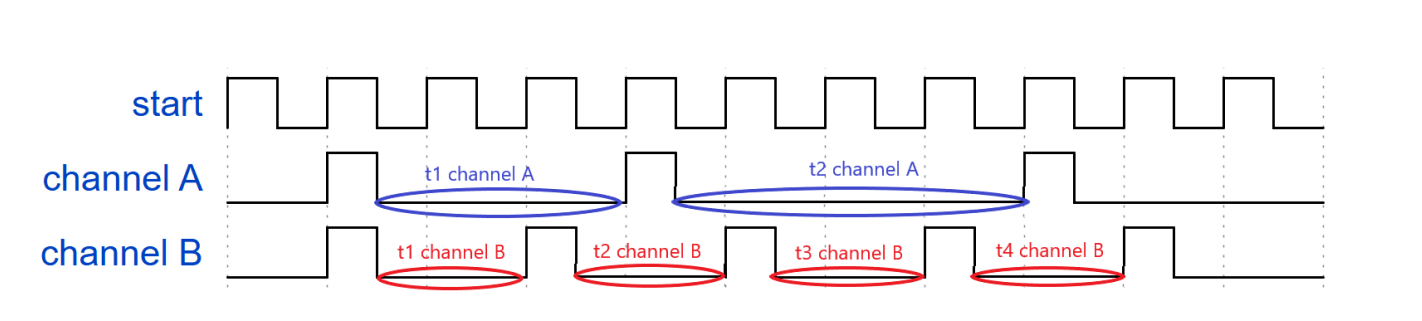
\includegraphics[width=6.23017in,height=1.52039in]{images/settings-for-signal-measurement-01.png}
\label{fig:52}
\end{figure}

The signal clearly shows the periodic start pulse that must be emitted,
along with two sets of pulse measurements recorded on Channel A (blue)
and Channel B (red), respectively. For Channel A, the software
identifies the times t1 Channel A and t2 Channel A. To obtain t1, it
subtracts the timestamp of pulse 1 from pulse 2, and for t2, it
subtracts pulse 2 from pulse 3. Then, the software calculates the
average between these two values, obtains their inverse, and converts
the result into seconds. For Channel B, the same procedure is followed:
the average is calculated between t1 Channel B, t2 Channel B, t3 Channel
B, and t4 Channel B, then the inverse is obtained, and the result is
converted to seconds. This final value is reported as the measurement
result.

The Tempico device has a 4-millisecond window to receive a stop pulse
after a start pulse is received. Additionally, it is essential that at
least two pulses are detected after the start pulse during the
measurement process, as otherwise it will not be possible to calculate
the time differences between pulses. Therefore, the input signal must
have a minimum frequency of 500 pulses per second for the software to
accurately estimate the counts.

\hypertarget{settings-before-measurement}{%
\subsubsection{Settings before
measurement}\label{settings-before-measurement}}

For this functionality, users can configure the channels on which the
count estimation will be performed, as well as choose from different
types of graphical displays. The merge option overlays the curves of all
channels on a single graph; separated creates an individual graph for
each channel; and detached opens each graph in a separate, resizable
dialog window. Additionally, the detached table option displays the
temporal count history in an independent dialog. The time range
parameter allows users to define the time intervals over which the
measurement graph will be displayed.

It is important to note that not all settings become locked once the
measurement begins. The only configuration that becomes restricted is
channel selection, which prevents enabling channels that were not
selected prior to starting the measurement. All other settings can be
adjusted dynamically while the measurement is running. The following
figure shows the configuration panel for these options.

\begin{figure}[H]
\centering
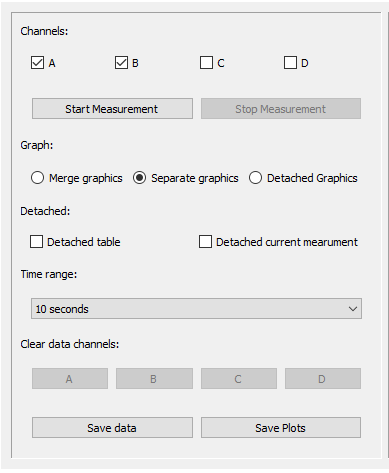
\includegraphics[width=4.05265in,height=4.92777in]{images/settings-before-measurement-01.png}
\label{fig:53}
\end{figure}

Once the user starts the measurement, the system automatically
determines the number of stops required to begin count estimation. This
step is critical, as configuring the Tempico device with several stops
greater than the actual number of pulses received after a start pulse
would result in no valid measurements being detected. To prevent this
issue, the software analyzes the incoming signal behavior and
automatically adjusts the appropriate number of stops before starting
the counting process.

\begin{figure}[H]
\centering
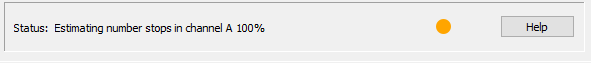
\includegraphics[width=6.1375in,height=0.65417in]{images/settings-before-measurement-02.png}
\label{fig:54}
\end{figure}

If the software detects that a channel is unable to register more than 2
stops, it will notify the user and prompt whether to stop the
measurement or continue with the remaining active channels. This
mechanism ensures user control over the process and helps prevent
unreliable results from channels with insufficient signal.

\begin{figure}[H]
\centering
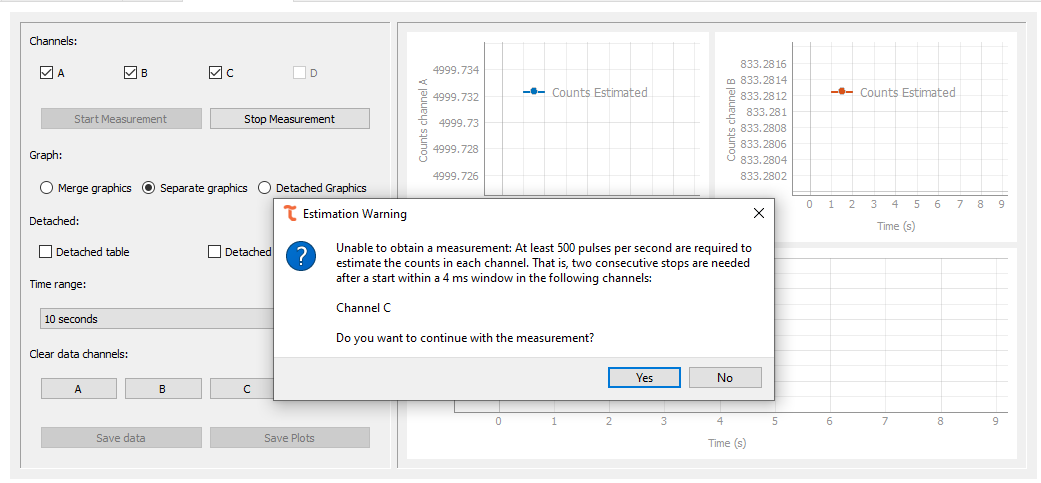
\includegraphics[width=6.1375in,height=2.84792in]{images/settings-before-measurement-03.png}
\label{fig:55}
\end{figure}

If the user chooses to continue the measurement, the channel for which
no valid data was found will be automatically disabled and cannot be
reselected unless the current measurement is stopped and a new one is
started. This ensures that only channels with valid signals are
considered during the estimation process.

\begin{figure}[H]
\centering
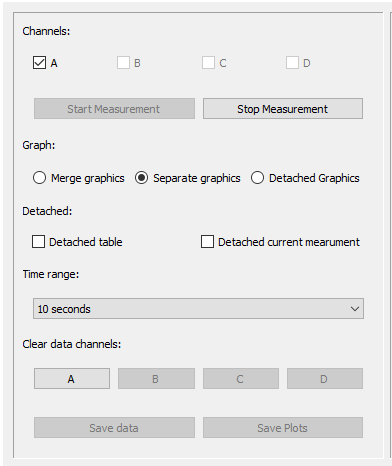
\includegraphics[width=3.45368in,height=4.10565in]{images/settings-before-measurement-04.png}
\label{fig:56}
\end{figure}

If the user chooses not to continue, the software will automatically
terminate the measurement, ensuring that no channels without valid
signals are processed.

\hypertarget{perform-a-measurement-2}{%
\subsubsection{Perform a measurement}\label{perform-a-measurement-2}}

To start the measurement, you must click the Start Measurement
(
\includegraphics[width=1.16683in,height=0.13601in]{images/perform-a-measurement-2-01.png}
) button, which will begin the stop number estimation process described
earlier. Once this process is complete, the measurement will begin to
run correctly.

First, we have the graphical section; if the Merge Graphics (

\includegraphics[width=0.71269in,height=0.13678in]{images/perform-a-measurement-2-02.png})
option is selected, all curves from the selected channels will be
displayed in a single chart.

\begin{figure}[H]
\centering
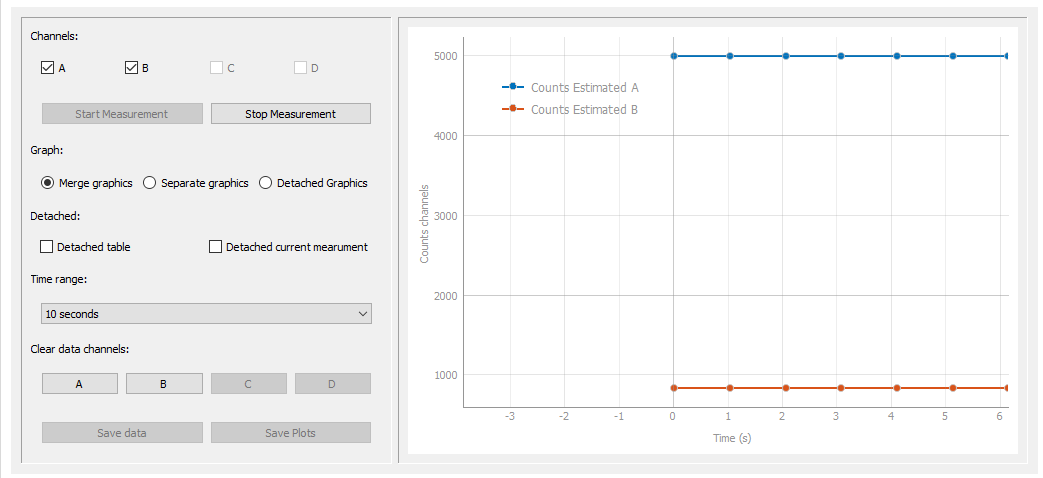
\includegraphics[width=6.1375in,height=2.8125in]{images/perform-a-measurement-2-03.png}
\label{fig:57}
\end{figure}

Whereas if the Separate Graphics
(
\includegraphics[width=0.84642in,height=0.22709in]{images/perform-a-measurement-2-04.png}
) option is selected, the curves for each channel will be displayed
individually, each in its own separate chart.

\begin{figure}[H]
\centering
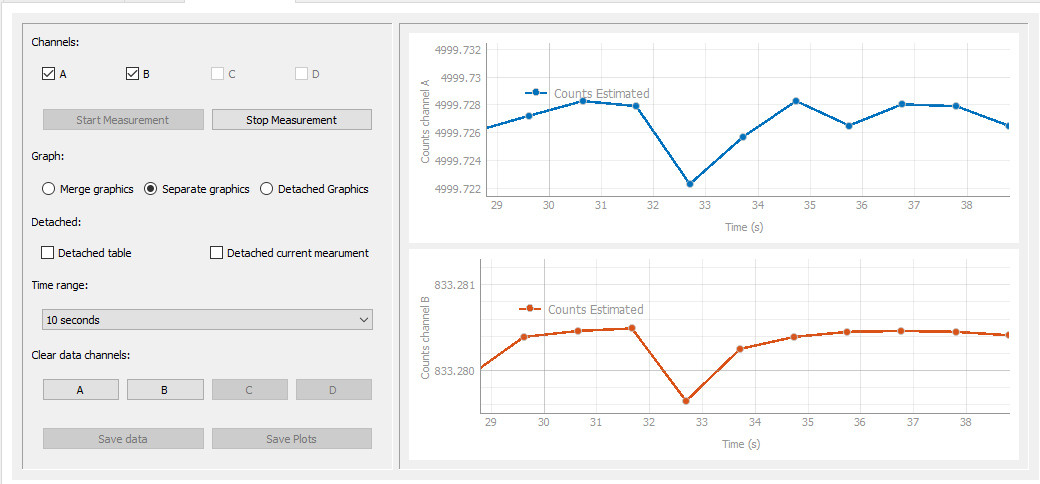
\includegraphics[width=6.1375in,height=2.85625in]{images/perform-a-measurement-2-05.png}
\label{fig:58}
\end{figure}

We also have the Detached Graphics
(
\includegraphics[width=0.74199in,height=0.25142in]{images/perform-a-measurement-2-06.png}
) option, which displays the graphs in separate dialog windows that open
independently from the main window.

\begin{figure}[H]
\centering
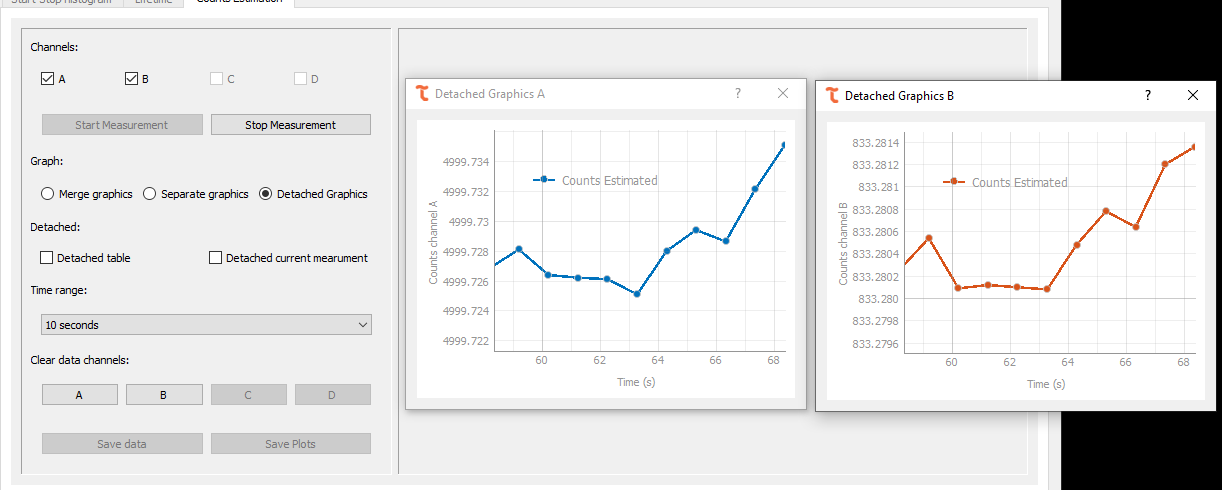
\includegraphics[width=6.1375in,height=2.46111in]{images/perform-a-measurement-2-07.png}
\label{fig:59}
\end{figure}

Time filters can be applied to the graphs using the Time Range dropdown
menu. This allows you to adjust the time range on the X-axis to view the
measurement history in detail. For example, if you select 50 seconds,
all graphs will display the last 50 seconds of the recorded data.

\begin{figure}[H]
\centering
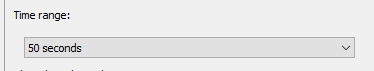
\includegraphics[width=3.83387in,height=0.73969in]{images/perform-a-measurement-2-08.png}
\label{fig:60}
\end{figure}

\begin{figure}[H]
\centering
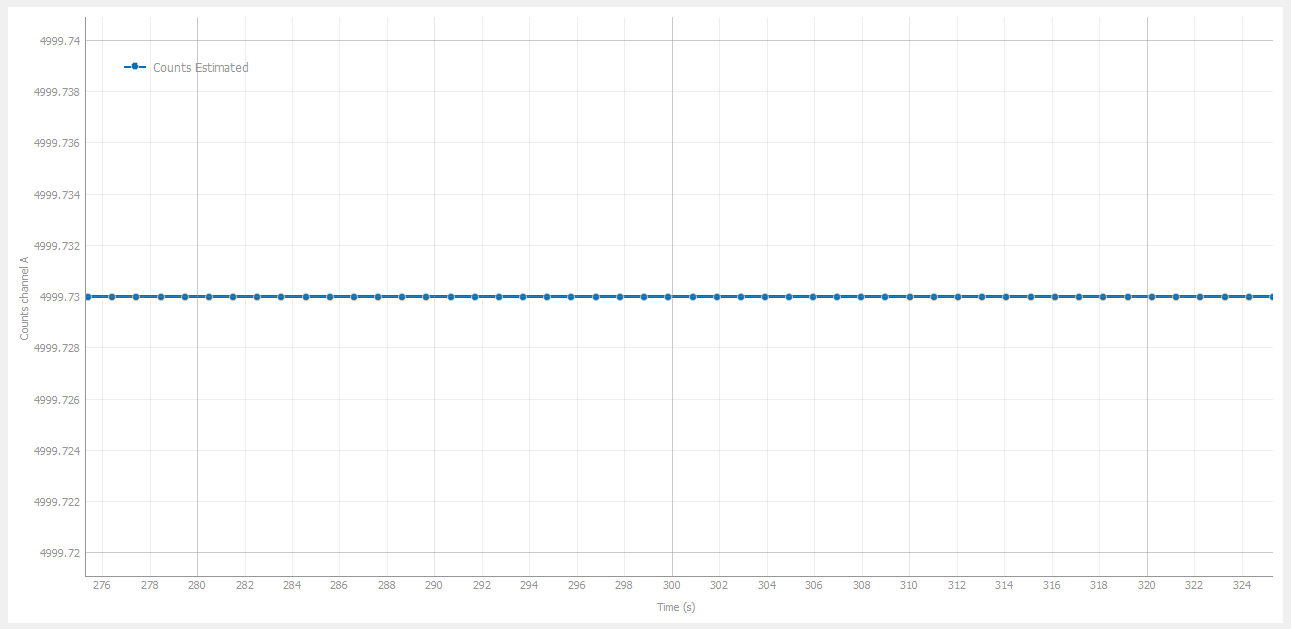
\includegraphics[width=6.1375in,height=2.99028in]{images/perform-a-measurement-2-09.png}
\label{fig:61}
\end{figure}

During the measurement, there is also a table section that displays the
history of the estimated count values along with the corresponding hour,
minutes, and seconds of registration. This section is located below the
graphs displayed on the screen.

\begin{figure}[H]
\centering
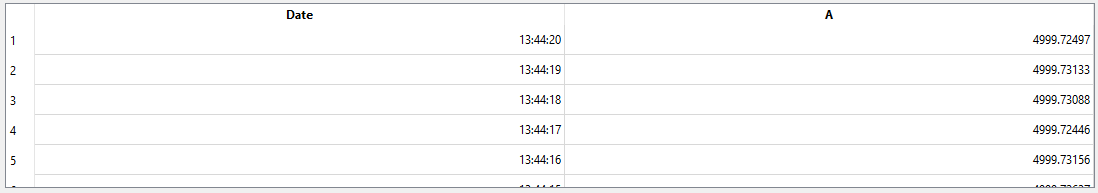
\includegraphics[width=6.1375in,height=1.07847in]{images/perform-a-measurement-2-10.png}
\label{fig:62}
\end{figure}

If the user wants to view the table more clearly, they can enable the
\emph{detached table} option available in the settings panel. This will
display the table in a separate dialog window, showing the same data as
the one at the bottom of the main window, but with enhanced detail.

\begin{figure}[H]
\centering

\includegraphics[width=5.78206in,height=1.08348in]{images/perform-a-measurement-2-11.png}
\label{fig:63}
\end{figure}

\begin{figure}[H]
\centering
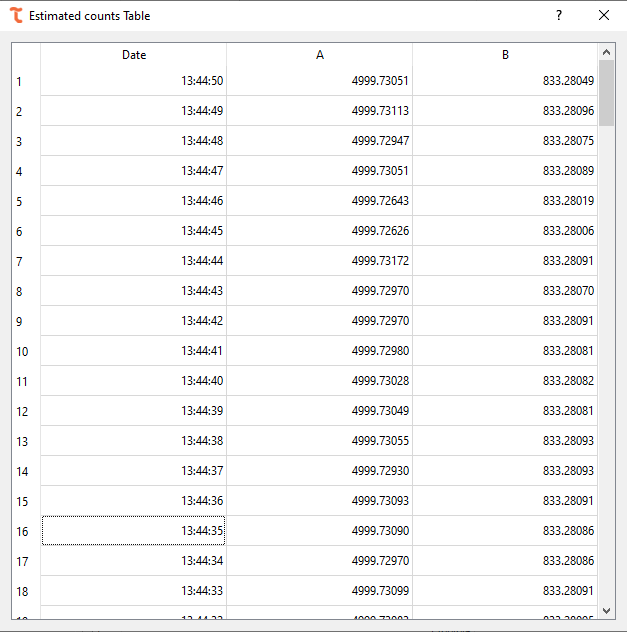
\includegraphics[width=3.89318in,height=3.92402in]{images/perform-a-measurement-2-12.png}
\label{fig:64}
\end{figure}

Likewise, in the bottom-left corner of the main window, the user can
view the value and the uncertainty corresponding to the most recently
reported measurement.

\begin{figure}[H]
\centering
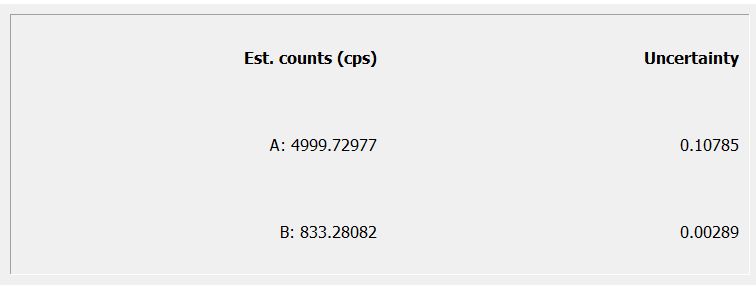
\includegraphics[width=6.1375in,height=2.32153in]{images/perform-a-measurement-2-13.png}
\label{fig:65}
\end{figure}

As before, the user can choose to view the current values in detached
mode by clicking the corresponding
checkbox.
\includegraphics[width=5.71955in,height=1.06265in]{images/perform-a-measurement-2-14.png}

After that, a separate dialog will open displaying the current
measurement values.

\begin{figure}[H]
\centering
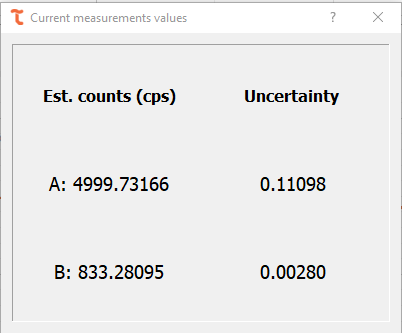
\includegraphics[width=4.18808in,height=3.43798in]{images/perform-a-measurement-2-15.png}
\label{fig:66}
\end{figure}

If a channel stops emitting values during the measurement process, the
software will notify the user through the status bar. Additionally, the
results table will display the message Low Counts, indicating that the
device is unable to perform the measurement because the number of
received counts is insufficient.

\begin{figure}[H]
\centering
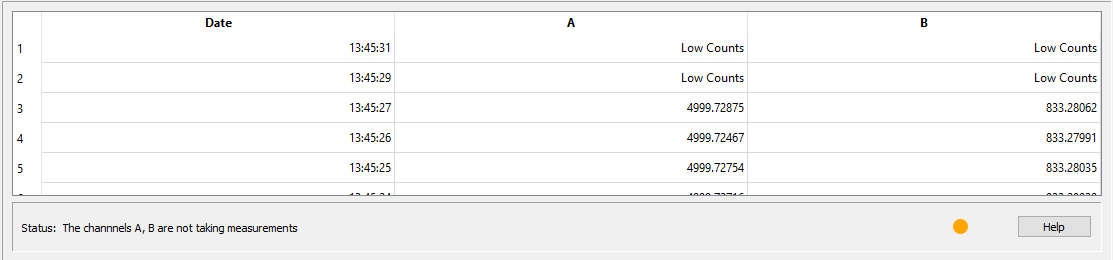
\includegraphics[width=6.1375in,height=1.43333in]{images/perform-a-measurement-2-16.png}
\label{fig:67}
\end{figure}

\begin{figure}[H]
\centering
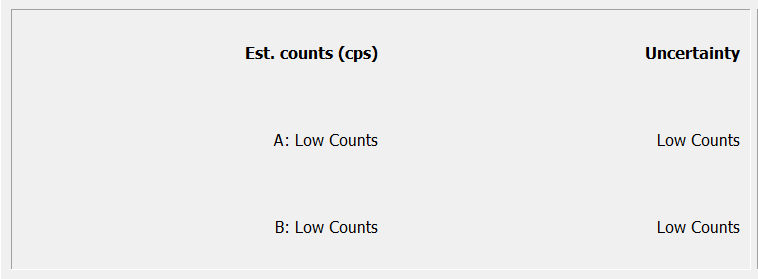
\includegraphics[width=6.1375in,height=2.25903in]{images/perform-a-measurement-2-17.png}
\label{fig:68}
\end{figure}

Once measurements are registered again on the channel, the process will
resume normally.

\hypertarget{save-data}{%
\subsubsection{Save data}\label{save-data}}

The user is responsible for deciding when to stop the measurement. To do
this, they must click the Stop Measurement
(
\includegraphics[width=1.54964in,height=0.1225in]{images/save-data-01.png}
) button. After this, the Save Data (

\includegraphics[width=1.41029in,height=0.1272in]{images/save-data-02.png})
button will be enabled, allowing the user to save the data in plain text
format. Upon clicking this button, a window like those used in other
functionalities will appear, prompting the user to choose the format in
which they wish to save the measurement.

\begin{figure}[H]
\centering
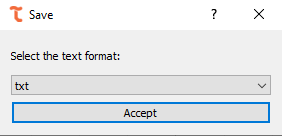
\includegraphics[width=2.93791in,height=1.41686in]{images/save-data-03.png}
\label{fig:69}
\end{figure}

Among the available formats for saving the data are .txt, .csv, and
.dat. Upon clicking Accept, a window will appear confirming that the
values have been successfully saved and displaying the path where the
files are located.

\begin{figure}[H]
\centering
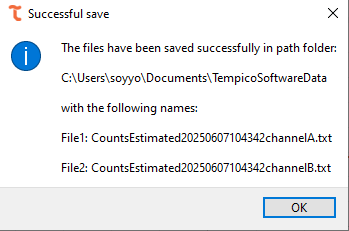
\includegraphics[width=3.63592in,height=2.40659in]{images/save-data-04.png}
\label{fig:70}
\end{figure}

The file will store both the timestamp of the recorded data and the
corresponding estimated count value.

\begin{figure}[H]
\centering
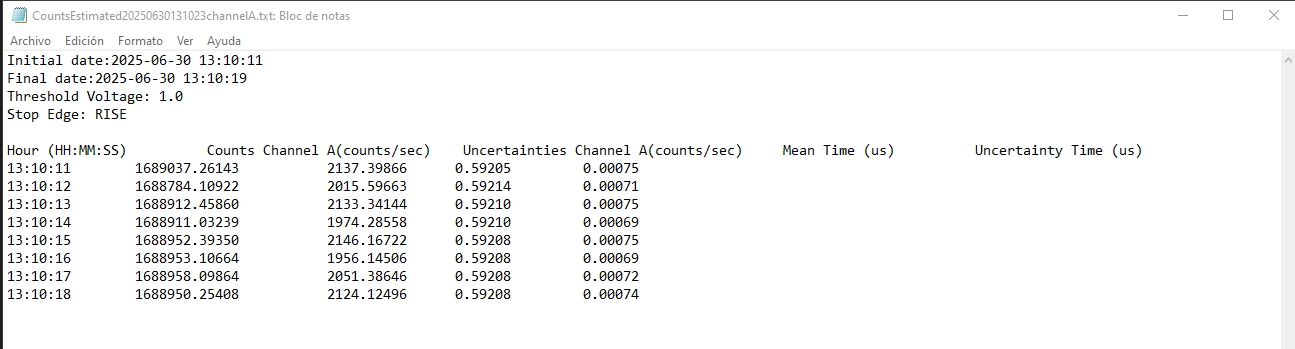
\includegraphics[width=6.1375in,height=1.65417in]{images/save-data-05.png}
\label{fig:71}
\end{figure}

\hypertarget{save-plot}{%
\subsubsection{Save plot}\label{save-plot}}

Similarly, once the measurement is completed, the option to save the
plots
(
\includegraphics[width=1.25924in,height=0.15546in]{images/save-plot-01.png})
will be enabled. As in the previous sections, a window will appear
allowing the user to select the format in which they wish to save the
graph, including PNG, TIFF, and JPG.

\begin{figure}[H]
\centering
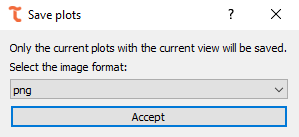
\includegraphics[width=3.11502in,height=1.42728in]{images/save-plot-02.png}
\label{fig:72}
\end{figure}

After clicking the accept button, a dialog window will open indicating
the path where the image was saved, including the file name and selected
format.

\begin{figure}[H]
\centering
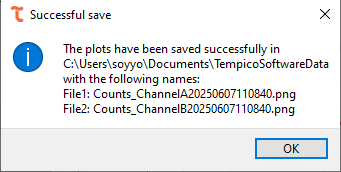
\includegraphics[width=3.55258in,height=1.79192in]{images/save-plot-03.png}
\label{fig:73}
\end{figure}

The graph will be saved exactly as it appears on screen. If the time
range filter has been applied, the image will reflect the corresponding
values on the X-axis. Additionally, if the graph has been visually
adjusted---either stretched or displayed with specific width-to-height
proportions---those proportions will be preserved when the graph is
saved.

\begin{figure}[H]
\centering
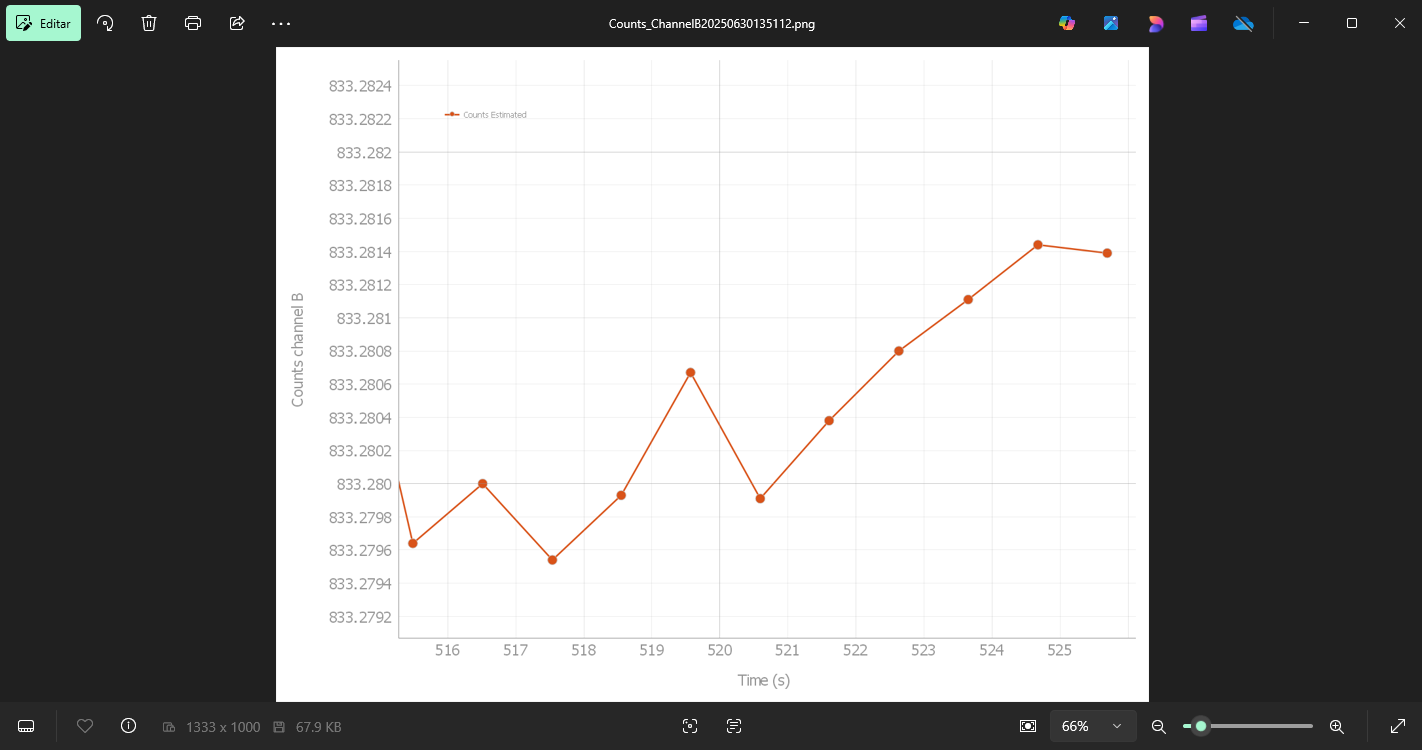
\includegraphics[width=4.6669in,height=2.46124in]{images/save-plot-04.png}
\label{fig:74}
\end{figure}

\hypertarget{time-stamping}{%
\subsection{Time stamping}\label{time-stamping}}

To comprehensively capture every pulse arriving at the start channel,
together with its corresponding stop pulses, while recording the precise
timestamp of each event, Tempico Software provides a measurement mode
optimized for fast and efficient data acquisition. This mode is
specifically designed to handle large data volumes.

\hypertarget{settings-before-measurements}{%
\subsubsection{Settings before
measurements}\label{settings-before-measurements}}

As with start-stop histogram measurements, any adjustment made in this
tab---whether through global settings or channel-specific
configurations---directly affects the measurement.

Before starting a measurement, users can select the channels on which
data will be recorded---options include channels A, B, C, or D.

\begin{figure}[H]
\centering
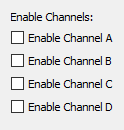
\includegraphics[width=1.29185in,height=1.35436in]{images/settings-before-measurements-01.png}
\label{fig:75}
\end{figure}

Users can also choose whether to display the measurement results table,
which may help reduce resource consumption. Furthermore, this option can
be enabled or disabled even after the measurement has already started.

\begin{figure}[H]
\centering

\includegraphics[width=0.85429in,height=0.29171in]{images/settings-before-measurements-02.png}
\label{fig:76}
\end{figure}

\hypertarget{manual-measurement}{%
\paragraph{Manual measurement}\label{manual-measurement}}

For this type of measurement, no prior parameters need to be configured;
the user simply clicks the Start Measurement button.

\begin{figure}[H]
\centering
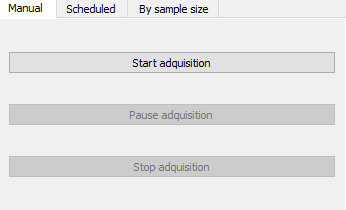
\includegraphics[width=3.60467in,height=2.18781in]{images/manual-measurement-01.png}
\label{fig:77}
\end{figure}

\hypertarget{scheduled-measurement}{%
\paragraph{Scheduled measurement}\label{scheduled-measurement}}

In this mode, the user specifies both the start time and the stop time
of the measurement. These values must be consistent with the system's
date and time settings. For instance, if a start date and time are set
in the past when the measurement begins, the program will display an
alert requesting the user to adjust the values. Similarly, if the stop
time is set earlier than the start time, a similar alert will be
generated.

\begin{figure}[H]
\centering
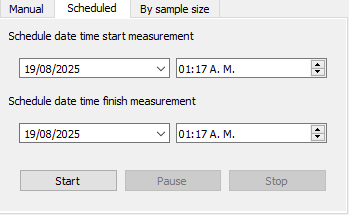
\includegraphics[width=3.63592in,height=2.2399in]{images/scheduled-measurement-01.png}
\label{fig:78}
\end{figure}

\hypertarget{by-sample-size-measurement}{%
\paragraph{By sample size
measurement}\label{by-sample-size-measurement}}

In this case, the user must define the number of measurements to be
recorded. Once this number is reached, data acquisition will
automatically stop.

\begin{figure}[H]
\centering
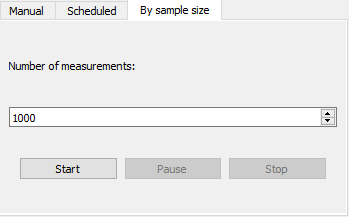
\includegraphics[width=3.63592in,height=2.26073in]{images/by-sample-size-measurement-01.png}
\label{fig:79}
\end{figure}

\emph{Note: If a start pulse is received without a corresponding stop
pulse, the software will still log it as a valid measurement and include
it in the dataset.}

\hypertarget{autosaving-measurements}{%
\paragraph{Autosaving measurements}\label{autosaving-measurements}}

The tab dedicated to handling large data volumes includes an autosave
feature, designed to prevent data loss in the event of system failures
or hardware limitations. This functionality allows data to be stored
automatically at user-defined intervals, as well as at the end of each
measurement.

The autosave interval can be freely configured. However, during the
saving process, acquisition is briefly paused (typically a few seconds
for short intervals, depending on the hardware). The available time
intervals are shown in the corresponding figure.

\begin{figure}[H]
\centering
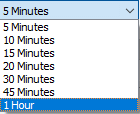
\includegraphics[width=1.45854in,height=1.18767in]{images/autosaving-measurements-01.png}
\label{fig:80}
\end{figure}

If an unexpected error occurs---such as an operating system failure,
hardware malfunction, or sudden shutdown/restart---data can be recovered
from the installation root directory of Tempico Software, inside the
TempData folder. This directory contains the file AutoSaveData.txt,
which stores all data recorded up to the last autosave. Although it is
not recommended to open this file directly, it can be used as a recovery
resource if necessary.

If autosave is disabled, users must manually click the Save Data button
at the end of the measurement to preserve results. This approach is
recommended for short acquisitions where every recorded value is
critical.

\begin{figure}[H]
\centering
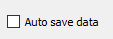
\includegraphics[width=1.17725in,height=0.40631in]{images/autosaving-measurements-02.png}
\label{fig:81}
\end{figure}

\emph{Technical considerations:}

\emph{When data is not immediately saved, it is temporarily stored in
RAM. In the 32-bit version of the software, memory usage is limited to 4
GB per process, regardless of the system's available resources. In the
64-bit version, the program can access all installed memory. It is
strongly recommended to keep autosave enabled, as the software can
acquire more than 2000 data points per second. For reference, storing 22
million data points in RAM requires approximately 4 GB of memory.}

\hypertarget{perform-a-measurement-3}{%
\subsubsection{Perform a measurement}\label{perform-a-measurement-3}}

Once the desired configuration has been completed, the measurement can
be started by pressing any of the start buttons corresponding to the
selected tab
(
\includegraphics[width=0.7in,height=0.14894in]{images/perform-a-measurement-3-01.png},
\includegraphics[width=2.68832in,height=0.14889in]{images/perform-a-measurement-3-02.png}).

If autosave is enabled, a window will pop up asking the user to select
the format in which the data should be saved.

\begin{figure}[H]
\centering
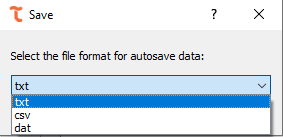
\includegraphics[width=2.94833in,height=1.42728in]{images/perform-a-measurement-3-03.png}
\label{fig:82}
\end{figure}

After confirming the format
(
\includegraphics[width=2.20663in,height=0.15576in]{images/perform-a-measurement-3-04.png})
in case autosave is enabled, or simply by pressing start if it is not,
the measurement will begin. The only exception is the scheduled
measurement, where a countdown will appear indicating the remaining time
before the measurement starts.

\begin{figure}[H]
\centering
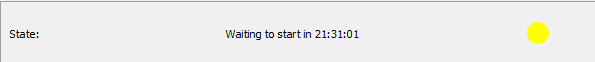
\includegraphics[width=6.1375in,height=0.63958in]{images/perform-a-measurement-3-05.png}
\label{fig:83}
\end{figure}

When this countdown is active, it is as if the software were already
running the measurement, since it is not possible to change the tab or
device configurations. If the user wishes to cancel the process before
it begins, they may do so by pressing the stop button
(
\includegraphics[width=0.7701in,height=0.14905in]{images/perform-a-measurement-3-06.png}).

Once started, the table will begin recording values. Start pulses will
be stored with year, month, day, hour, minute, and second format, with
microsecond resolution. Stop pulses will be stored with picosecond
resolution, along with the channel information that generated them, the
table will show only the last 50000 start stop and channel values.

\begin{figure}[H]
\centering
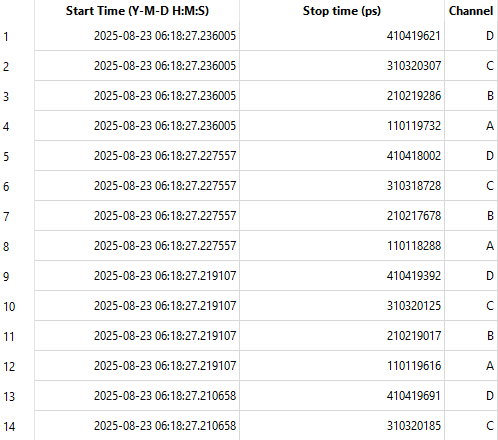
\includegraphics[width=5.18822in,height=4.58397in]{images/perform-a-measurement-3-07.png}
\label{fig:84}
\end{figure}

For the Tempico TP1200 versions, it is possible to obtain negative
measurements with a range of down to --200 ns.

\begin{figure}[H]
\centering
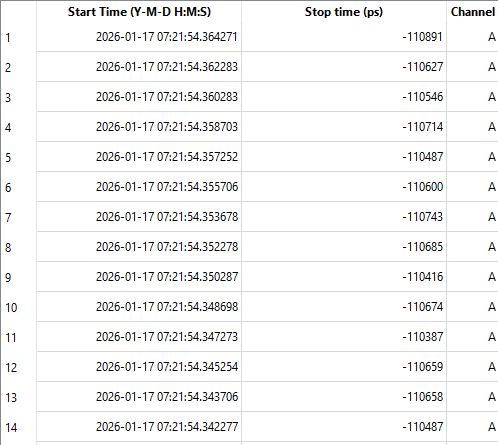
\includegraphics[width=5.18822in,height=4.63606in]{images/perform-a-measurement-3-08.png}
\label{fig:85}
\end{figure}

The panel in the lower-left corner will display the total number of
measurements recorded per channel, as well as the overall total.

\begin{figure}[H]
\centering
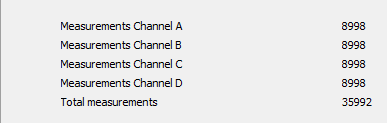
\includegraphics[width=4.03181in,height=1.28143in]{images/perform-a-measurement-3-09.png}
\label{fig:86}
\end{figure}

The status bar will indicate whether the measurement is running
correctly or if there is an issue with the selected channels.

\begin{figure}[H]
\centering

\includegraphics[width=6.1375in,height=0.6125in]{images/perform-a-measurement-3-10.png}
\label{fig:87}
\end{figure}

\begin{figure}[H]
\centering

\includegraphics[width=6.1375in,height=0.63958in]{images/perform-a-measurement-3-11.png}
\label{fig:88}
\end{figure}

It will also show progress depending on the measurement type. For
scheduled measurements, the status bar will display the remaining time
until completion.

\begin{figure}[H]
\centering

\includegraphics[width=6.1375in,height=0.65278in]{images/perform-a-measurement-3-12.png}
\label{fig:89}
\end{figure}

For sample-size-based measurements, it will show the progress percentage
according to the number of acquired records compared to the expected
amount.

\begin{figure}[H]
\centering
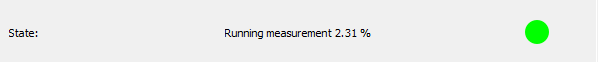
\includegraphics[width=6.1375in,height=0.63611in]{images/perform-a-measurement-3-13.png}
\label{fig:90}
\end{figure}

When autosave is in process, the status bar will display the message
saving data. The duration of this message corresponds to the time during
which the software pauses acquisition to save the accumulated data.

The measurement can also be paused by clicking the Pause
(
\includegraphics[width=2.0in,height=0.1in]{images/perform-a-measurement-3-14.png}, 
\includegraphics[width=0.76in,height=0.14in]{images/perform-a-measurement-3-15.png})
button. This option allows the user to temporarily stop the measurement
without starting a new one or losing the data already recorded. It is
particularly useful when a connection needs to be adjusted in the timer
without restarting the entire process.

\begin{figure}[H]
\centering

\includegraphics[width=6.08418in,height=0.63551in]{images/perform-a-measurement-3-16.png}
\label{fig:91}
\end{figure}

At the end of the measurement, the status bar will indicate that the
data is being processed. During this step, the information is saved in
the path selected by the user and the records are organized.

\begin{figure}[H]
\centering

\includegraphics[width=6.1375in,height=0.65208in]{images/perform-a-measurement-3-17.png}
\label{fig:92}
\end{figure}

In any type of measurement, it is possible to manually stop the process
at any time by pressing the stop button
(
\includegraphics[width=2.52909in,height=0.1566in]{images/perform-a-measurement-3-18.png},

\includegraphics[width=0.7701in,height=0.14905in]{images/perform-a-measurement-3-06.png}).

If autosave was enabled, at the end of the process a window will pop up
confirming that the measurement was successfully saved and showing the
path where the file was stored.

\begin{figure}[H]
\centering
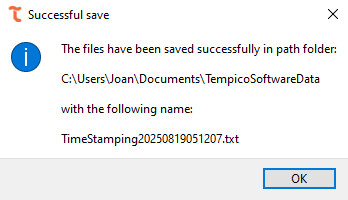
\includegraphics[width=3.30698in,height=1.90057in]{images/perform-a-measurement-3-19.png}
\label{fig:93}
\end{figure}

\hypertarget{save-data-1}{%
\subsubsection{Save data}\label{save-data-1}}

For the time stamping functionality, the user can only save the data
generated by the software. This process begins when clicking on the Save
Data button, which is only enabled if the Auto Save checkbox is not
selected. Once pressed, a dialog window appears, allowing the user to
choose the file extension with its corresponding format. The available
options are .txt, .csv, or .dat.

\begin{figure}[H]
\centering
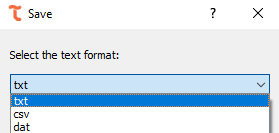
\includegraphics[width=2.90666in,height=1.38561in]{images/save-data-1-01.png}
\label{fig:94}
\end{figure}

If the user previously had the Auto Save option enabled and attempts to
save the data again using the same format initially selected, the
software will display an alert notifying that the data has already been
saved.

\begin{figure}[H]
\centering
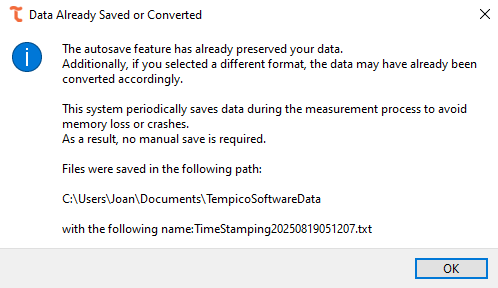
\includegraphics[width=4.03425in,height=2.33306in]{images/save-data-1-02.png}
\label{fig:95}
\end{figure}

If the user chooses a different file extension, the data will be saved
again, but this time in the new format specified in the dialog window.

\begin{figure}[H]
\centering
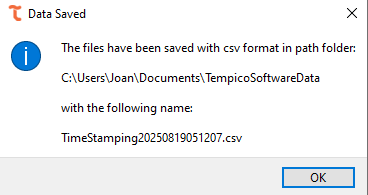
\includegraphics[width=2.96349in,height=1.57033in]{images/save-data-1-03.png}
\label{fig:96}
\end{figure}

When the Auto Save option is not enabled, the software displays an
additional dialog window indicating the percentage of progress during
the data processing stage.

\begin{figure}[H]
\centering
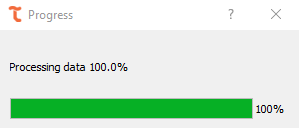
\includegraphics[width=2.50614in,height=1.07286in]{images/save-data-1-04.png}
\label{fig:97}
\end{figure}

At this point, the data is sorted and subsequently saved in the desired
path defined by the user. Finally, once the operation is completed, a
confirmation dialog---similar to the one shown previously---appears to
indicate that the data has been successfully stored.

The file that stores the data within the header includes the
configurations applied to each channel at the time the measurement was
performed. This file is organized into three columns: the first
corresponds to the \textbf{start} value, represented in the format
year-month-day-hour-minutes-seconds; the second contains the
\textbf{stop} value, which is expressed in \textbf{picoseconds}; and the
third identifies the \textbf{channel} in which the measurement was
recorded. In this way, the information is structured and linked both to
the temporal start point and to the corresponding channel.

\begin{figure}[H]
\centering
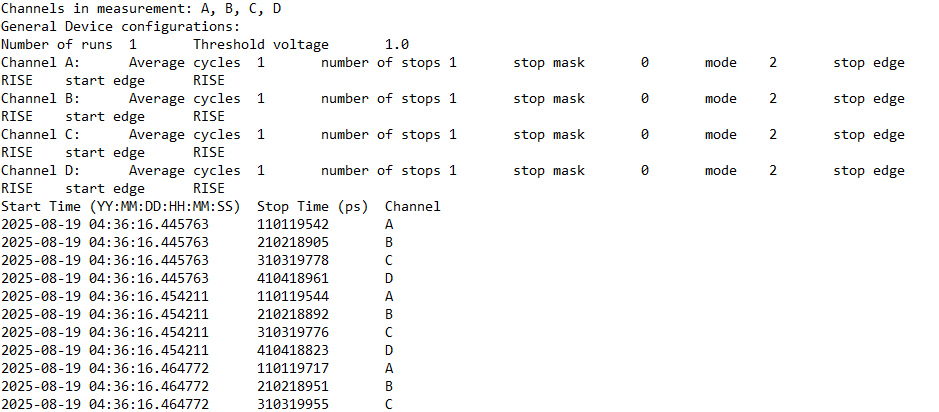
\includegraphics[width=6.13853in,height=2.69351in]{images/save-data-1-05.png}
\label{fig:98}
\end{figure}

\hypertarget{autocorrelation-fluorescence-correlation-spectroscopy}{%
\subsection{Autocorrelation (Fluorescence Correlation
Spectroscopy)}\label{autocorrelation-fluorescence-correlation-spectroscopy}}

The Autocorrelation (FCS) tab allows the user to compute the normalized
intensity autocorrelation function G($\tau$) from the stop timestamps
recorded on a single channel, which is the basis of Fluorescence
Correlation Spectroscopy (FCS) experiments. From the shape of this
curve, parameters such as the diffusion time, the number of particles in
the observation volume or the presence of chemical or triplet-state
dynamics can be estimated through curve fitting.

\hypertarget{settings-before-measurements-1}{%
\subsubsection{Settings before
measurements}\label{settings-before-measurements-1}}

The input signal connected to the stop channel must satisfy a minimum
requirement: at least 2 stop pulses per start cycle must be received.
This is because the software discards the first stop of every cycle,
using it only as a time reference, and computes the actual inter-photon
intervals from the second stop onward; if fewer than 2 valid stops are
received in a cycle, that cycle contributes no data to the correlation
curve.

\begin{figure}[H]
\centering
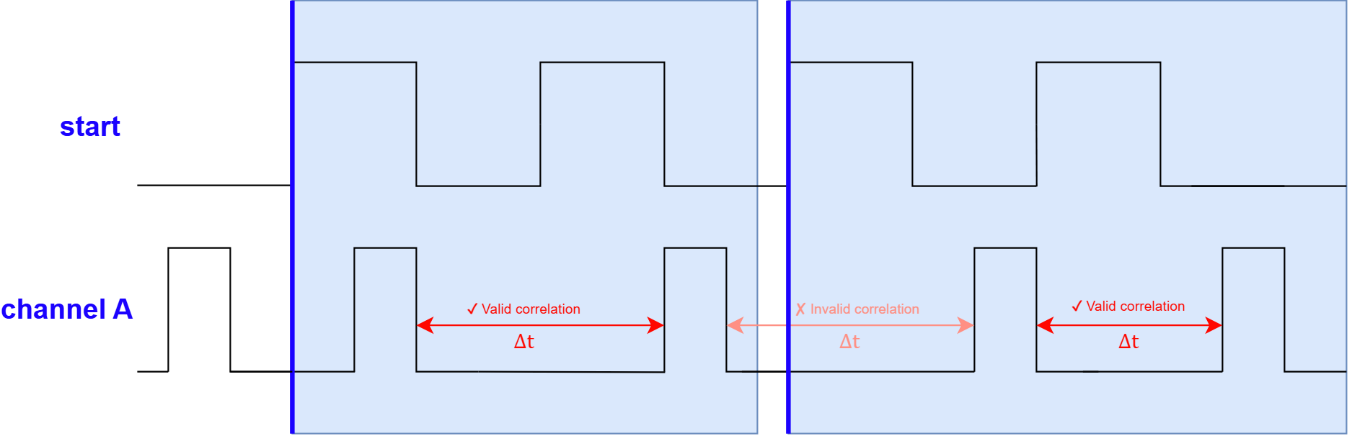
\includegraphics[width=6.1375in,height=2.00625in]{images/settings-before-measurements-1-01.png}
\label{fig:99}
\end{figure}

Regarding the acquisition settings, the user must configure the
following correlator parameters, located on the left panel of the tab.
The Stop Channel dropdown selects the channel (A, B, C, or D) whose
timestamps will be correlated. The Base bin width $\tau$\textsubscript{0}
field sets, in microseconds, the shortest lag time of the multiple-tau
correlator, and can be figured from 1 $\mu$s up to 10,000,000 $\mu$s; this value
should be chosen according to the expected diffusion or relaxation times
of the sample, since a base bin width that is too large may not resolve
fast dynamics, while one that is too small may unnecessarily increase
the noise at short lag times. Finally, the user can either set a fixed
Duration, from 1 second up to 24 hours, or enable the Continuous
measurement checkbox, which ignores the duration value and keeps the
correlation running until the user presses Stop.

\begin{figure}[H]
\centering
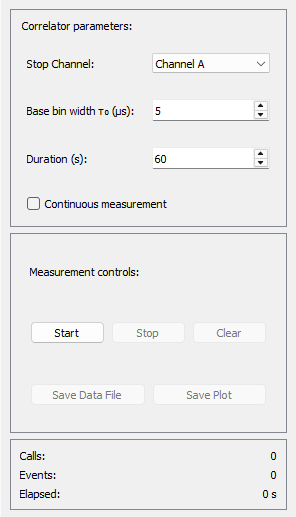
\includegraphics[width=3.08376in,height=5.38617in]{images/settings-before-measurements-1-02.png}
\label{fig:100}
\end{figure}

\hypertarget{perform-a-measurement-4}{%
\subsubsection{Perform a measurement}\label{perform-a-measurement-4}}

Once the desired configuration is selected, click the Start button to
begin the acquisition. While the measurement is running, the Stop
Channel, the Base bin width $\tau$\textsubscript{0}, the Duration, and the
Continuous measurement option are locked and cannot changed. The
autocorrelation curve G($\tau$) is plotted live against $\tau$ on a logarithmic
time axis as new data arrives. At any point the user can press Clear to
reset the curve, or Stop to end the measurement before the configured
duration elapses.

\begin{figure}[H]
\centering
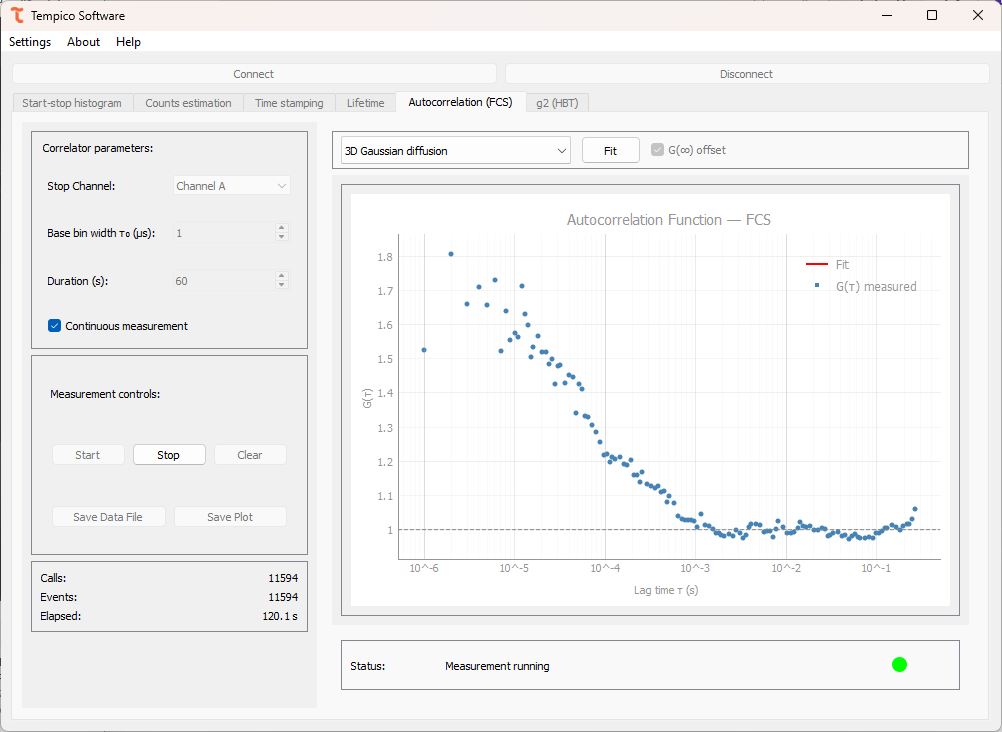
\includegraphics[width=6.13750in,height=4.48333in]{images/perform-a-measurement-4-01.png}
\label{fig:103}
\end{figure}

The panel below settings reports the acquisition progress through three
values: Calls, which indicates the number of calls made to the device
since the measurement started; Events, which indicates the number of
valid stop events detected on the selected channel since the measurement
started; and Elapsed, which indicates the elapsed time since the
measurement started, shown in seconds and, if applicable, against the
total configuration duration.

\begin{figure}[H]
\centering
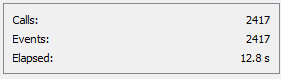
\includegraphics[width=2.93056in,height=0.82569in]{images/perform-a-measurement-4-02.png}
\label{fig:104}
\end{figure}

Next to this panel, the Status bar shows a colored dot together with a
short descriptive message, which the user should monitor throughout the
measurement. A grey dot indicates that no measurement is currently
running. A green dot indicates that the measurement is running normally,
with the message reporting the current number of calls, events and
elapsed time. An orange dot indicates that a warning condition was
detected; the message ``No measurements in Start Channel'' means that
the device is not receiving any start pulses, while the message ``No
measurements in Stop Channel {[}A/B/C/D{]}'' means that no valid pulses
are being detected on the selected stop channel. If either warning
persists, the user should check the corresponding cable connections and
the signal levels before continuing the measurement.

\begin{figure}[H]
\centering
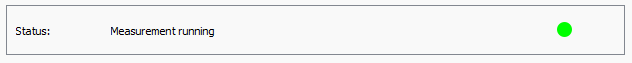
\includegraphics[width=6.13750in,height=0.60764in]{images/perform-a-measurement-4-03.png}
\label{fig:105}
\end{figure}

\begin{figure}[H]
\centering
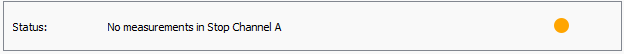
\includegraphics[width=6.08140in,height=0.52226in]{images/perform-a-measurement-4-04.png}
\label{fig:106}
\end{figure}

\hypertarget{post-measurement}{%
\subsubsection{Post-measurement}\label{post-measurement}}

\hypertarget{fitting-1}{%
\paragraph{Fitting}\label{fitting-1}}

Once the measurement finishes, the user can fit the measured curve to
one of six correlation models available in the fit model dropdown,
located in the upper-right panel. Selecting a model updates the equation
shown above the parameter table, which list an editable Initial value
column and a read-only Fit result column. The Auto button restores the
initial guesses automatically suggested by the software for the selected
model, and the G($\infty$) offset checkbox adds a constant baseline term to the
fitted equation of any model.

Clicking Fit runs the fit and fills the Fit result column; the fitting
curve is the overlaid on the plot, distinguished by the Fit and G($\tau$)
measured legend entries. If a reliable value cannot be estimated, the
software reports ``nan'' for the parameter. Since the quality of the fit
depends on the initial guesses, the user is free to edit them manually
in the Initial value column before running the fit again, or restore the
software's suggested values with the Auto button.

\begin{figure}[H]
\centering
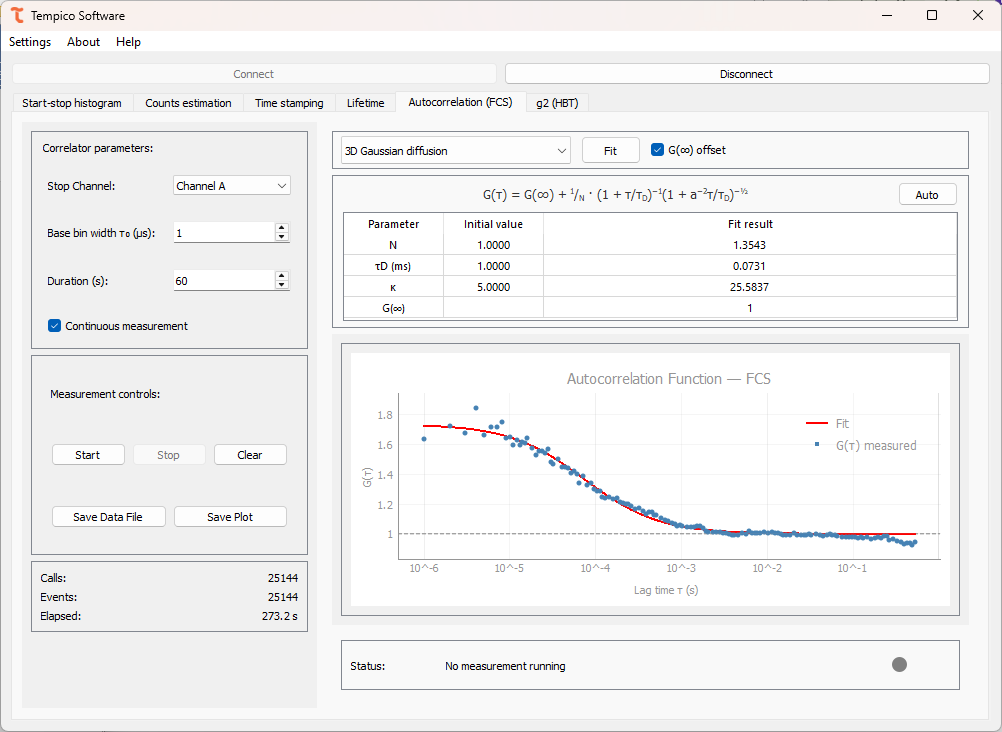
\includegraphics[width=6.13750in,height=4.48333in]{images/fitting-1-01.png}
\label{fig:107}
\end{figure}

\hypertarget{gaussian-diffusion}{%
\subparagraph{Gaussian diffusion}\label{gaussian-diffusion}}

\[G(\infty) + \frac{1}{N} \cdot \left( 1 + \frac{\tau}{\tau_{0}} \right)^{- 1} \cdot \left( 1 + a^{- 2}\frac{\tau}{\tau_{0}} \right)^{- \frac{1}{2}}\]

Describes a singles species diffusing freely in three dimensions through
a Gaussian observation volume, The fitted parameters are N, the average
number of particles in the observation volume.

\hypertarget{anomalous-diffusion}{%
\subparagraph{Anomalous diffusion}\label{anomalous-diffusion}}

\[G(\infty) + \frac{1}{N} \cdot \left( 1 + \left( \frac{\tau}{\tau_{D}} \right)^{a} \right)^{- 1} \cdot \left( 1 + a^{- 2}\left( \frac{\tau}{\tau_{D}} \right)^{a} \right)^{- \frac{1}{2}}\]

Extends the 3D Gaussian diffusion model to account for non-Brownian,
anomalous transport. In addition to N, $\tau$\textsubscript{D} (ms), and $\kappa$,
it includes the anomaly exponent $\alpha$ which equals 1 for normal diffusion
and deviates from 1 when the diffusion is sub- or super-diffusive.

\hypertarget{chemical-relaxation}{%
\subparagraph{Chemical relaxation}\label{chemical-relaxation}}

\[\ \ \ \ G(\infty) + \frac{1}{N} \cdot K \cdot \exp\left\lbrack - \frac{\tau}{\tau_{B}} \right\rbrack\ \ \ \ \ \ \ \ \left\lbrack G(0) = \frac{K}{N},\ \ K = \frac{k_{on}}{k_{off}} \right\rbrack\]

Describes a two-state chemical equilibrium, such as binding/unbinding or
blinking, rather than diffusion. The fitted parameters are N, the
relaxation time $\tau$\textsubscript{B}, in ms, and K, the ratio between the
on- and off-rate constants of the reaction (K =
k\textsubscript{on}/k\textsubscript{off}).

\hypertarget{diffusion-with-flow}{%
\subparagraph{Diffusion with flow}\label{diffusion-with-flow}}

\[G(\infty) + \frac{1}{N} \cdot \left( 1 + \frac{\tau}{\tau_{D}} \right)^{- 1} \cdot \left( 1 + a^{- 2}\frac{\tau}{\tau_{D}} \right)^{- \frac{1}{2}} \cdot \exp\left\lbrack - \frac{\left( \frac{\tau}{\tau_{v}} \right)^{2}}{1 + \frac{\tau}{\tau_{D}}} \right\rbrack\]

Combines 3D Gaussian diffusion with a directional flow term, useful when
the sample is subject to a net drift, such as in a microfluidic channel.
The fitted parameters are N, $\tau$\textsubscript{D} (ms). The structure
parameter a, and the flow time $\tau$\textsubscript{v}, in ms, which
represents the average transit time of a particle across the observation
volume due to flow.

\hypertarget{triplet-state-correction}{%
\subparagraph{Triplet state
correction}\label{triplet-state-correction}}

\[G(\infty) + \frac{1}{N} \cdot \frac{1 - F + F \cdot \exp\left\lbrack - \frac{\tau}{\tau_{F}} \right\rbrack}{1 - F} \cdot \left( 1 + \frac{\tau}{\tau_{D}} \right)^{- 1} \cdot \left( 1 + a^{- 2}\frac{\tau}{\tau_{D}} \right)^{- \frac{1}{2}}\]

Adds a photophysical blinking term to the 3D Gaussian diffusion model,
accounting for fluorophores transiently entering a non-fluorescent
triplet state. The fitted parameters are N, $\tau$\textsubscript{D} (ms), the
structure parameter a, the triplet fraction F, which represents the
proportion of molecules in the triplet state, and the triplet relaxation
time $\tau$\textsubscript{F}, in $\mu$s.

\hypertarget{two-component-diffusion}{%
\subparagraph{Two-component diffusion}\label{two-component-diffusion}}

\(G(\infty) + \frac{1}{N} \cdot \left( {a_{1} \cdot \left( 1 + \frac{\tau}{\tau_{D1}} \right)}^{- 1} \cdot \left( 1 + a^{- 2}\frac{\tau}{\tau_{D1}} \right)^{- \frac{1}{2}} + {a_{2} \cdot \left( 1 + \frac{\tau}{\tau_{D2}} \right)}^{- 1} \cdot \left( 1 + a^{- 2}\frac{\tau}{\tau_{D2}} \right)^{- \frac{1}{2}} \right)\)

Models two diffusing species with different mobilities, such as free dye
and dye bound to a larger complex. The fitted parameters are N, the
diffusion times of each species $\tau$\textsubscript{D1} and
$\tau$\textsubscript{D2}, in ms, the amplitude fraction of the first species
$\alpha$\textsubscript{1}, and the structure parameter a.

\hypertarget{save-data-2}{%
\paragraph{Save data}\label{save-data-2}}

Once the measurement finishes, the Save Data File button is enabled.
Clicking it opens a dialog window where the user selects the file
format: .txt, .csv, or .dat. Two files are generated: one containing the
$\tau$/G($\tau$) pairs of the autocorrelation curve, and another with the
measurement window, the device model, the correlator parameters, and the
selected stop channel; if a fit was performed, the fit model, its
equation, and the resulting parameters values are also included in the
leader.

\begin{figure}[H]
\centering
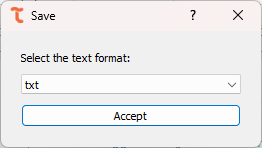
\includegraphics[width=2.8in,height=2.54in]{images/save-data-2-01.png}
\label{fig:108}
\end{figure}

\begin{figure}[H]
\centering
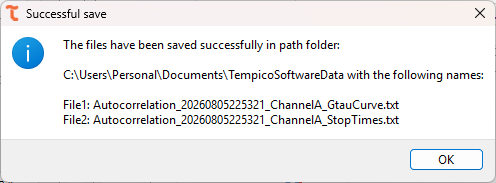
\includegraphics[width=5.16739in,height=1.90652in]{images/save-data-2-02.png}
\label{fig:109}
\end{figure}

\begin{figure}[H]
\centering
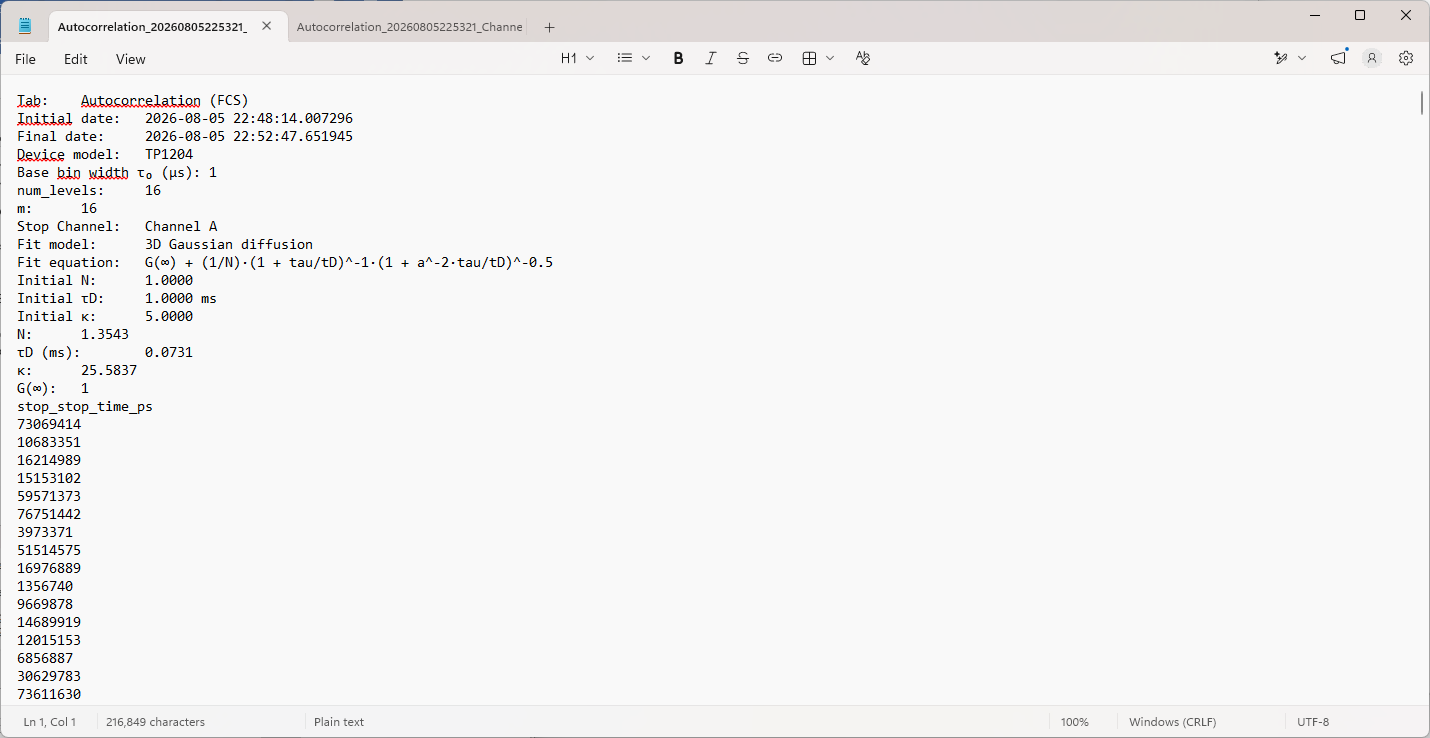
\includegraphics[width=5.94097in,height=3.06594in]{images/save-data-2-03.png}
\label{fig:110}
\end{figure}

\begin{figure}[H]
\centering
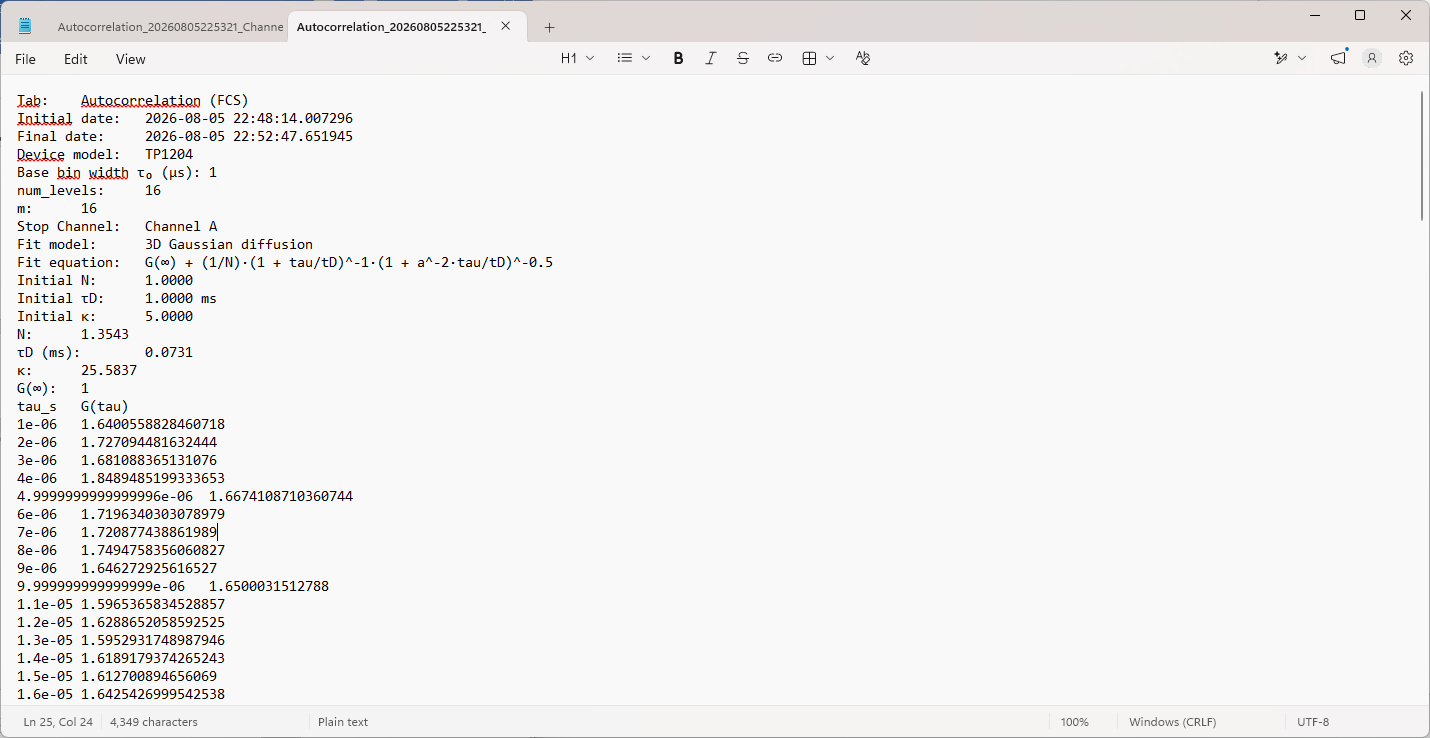
\includegraphics[width=6.04399in,height=3.11910in]{images/save-data-2-04.png}
\label{fig:111}
\end{figure}

Likewise, the Save Plot button exports the graph exactly as it appears
in screen, including the fitted curve if one was calculated. The
available formats are .png, .tiff, and .jpg. In both cases, once the
user selects the desired format and confirms, a confirmation window
appears indicating that the file was saved successfully and displaying
the path where it was stored.

\begin{figure}[H]
\centering
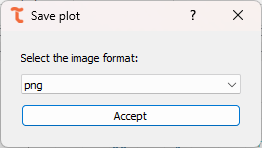
\includegraphics[width=3.0in,height=2.6in]{images/save-data-2-05.png}
\label{fig:112}
\end{figure}

\begin{figure}[H]
\centering
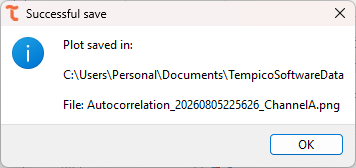
\includegraphics[width=3.70885in,height=1.75024in]{images/save-data-2-06.png}
\label{fig:113}
\end{figure}

\begin{figure}[H]
\centering
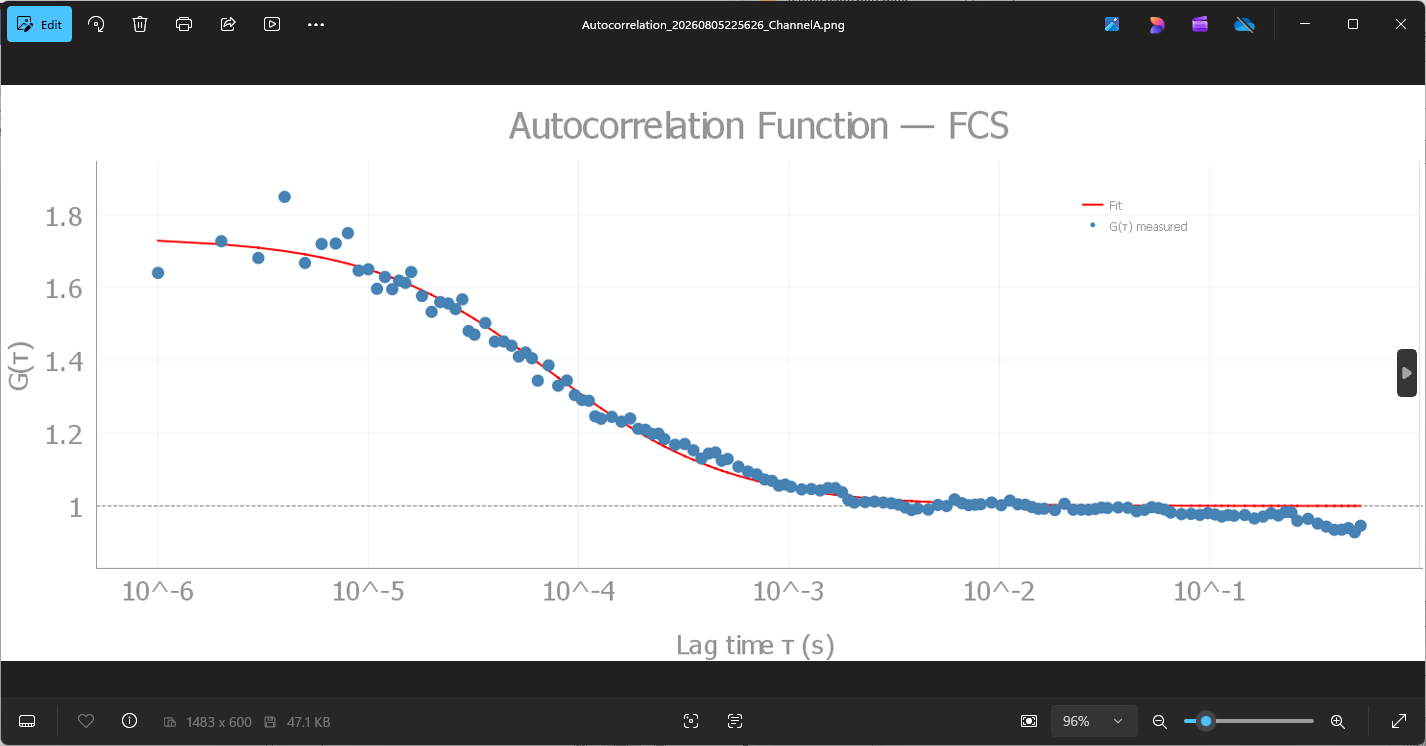
\includegraphics[width=6.13750in,height=2.40752in]{images/save-data-2-07.png}
\label{fig:114}
\end{figure}

\hypertarget{g_2-hanbury-brown-and-twiss}{%
\subsection{\texorpdfstring{g\(_{}^{(2)}\) (Hanbury Brown and
Twiss)}{g\_\{\}\^{}\{(2)\} (Hanbury Brown and Twiss)}}\label{g_2-hanbury-brown-and-twiss}}

The g\textsuperscript{(2)}(HBT) tab allows the user to compute the
second-order intensity correlation function g\textsuperscript{(2)}($\tau$),
following a Hanbury Brown-Twiss (HBT) type measurement. The tab builds a
symmetric histogram of the delay $\tau$ between the start signal and the stop
signal recorded on a single channel, normalized so that uncorrelated
light gives g\textsuperscript{(2)}($\tau$) =1. The shape of this curve around
$\tau$=0 reveals the photon statistics of the light source: a dip indicates
photon antibunching, typical of single-photon emitters, while a peak
indicates bunching, typical of thermal or chaotic light sources.

\hypertarget{settings-before-measurements-2}{%
\subsubsection{Settings before
measurements}\label{settings-before-measurements-2}}

The g\textsuperscript{(2)}($\tau$) histogram requires only one valid stop
pulse per start cycle, since only the first stop of each cycle is used
to computed $\tau$. If the user wants the software to additionally estimate
the coincidence rate through the Count Estimation feature, at least 2
stops per cycle are needed so that a stop-to-stop time interval can be
computed; in that case, the software automatically requests the extra
stop from the device when the corresponding checkbox is enabled, with no
additional channel configuration required from the user.

\begin{figure}[H]
\centering
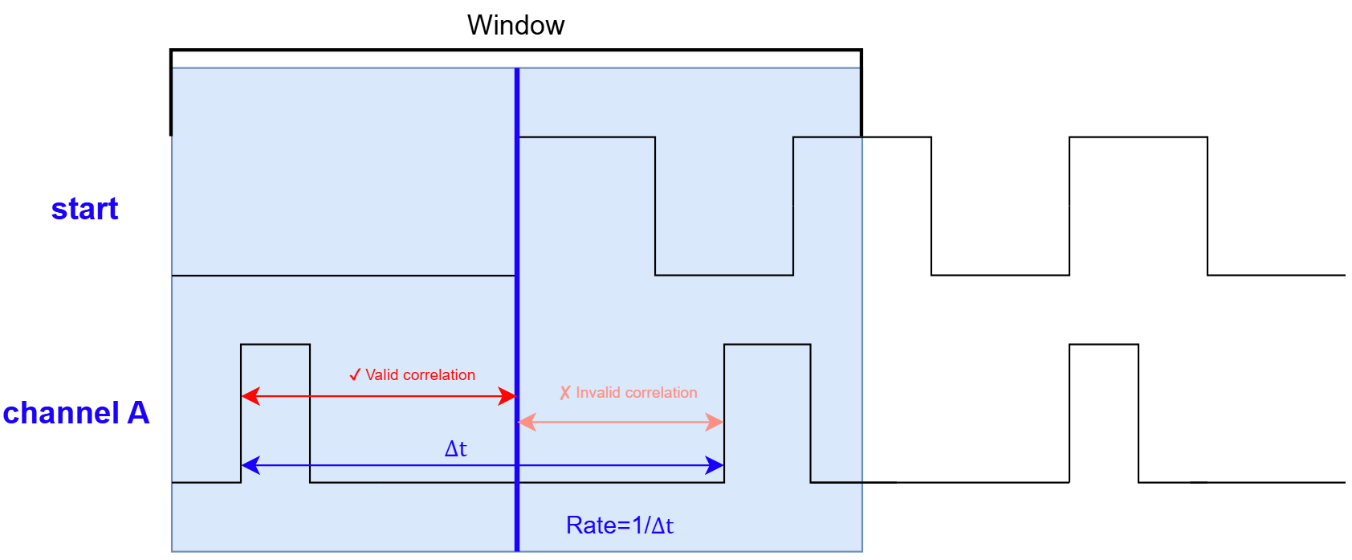
\includegraphics[width=6.1375in,height=2.54028in]{images/settings-before-measurements-2-01.png}
\label{fig:101}
\end{figure}

Regarding the acquisition settings, the user must configure the
following parameters, located on the left panel of the tab. The Stop
Channel dropdown selects the channel (A, B, C, or D) whose delay
relative to the start signal will be histogrammed. The Bin width field
sets, in nanoseconds, the width of each histogram bin, and can be
configured from 0.1 ns up to 10,000 ns. The Window ($\pm$) field sets, in
nanoseconds, the half-width of the histogram around $\tau$=0, and can be
configured from 10 ns up to 100,00 ns; together with the bin width, this
defines the total range and resolution of the g\textsuperscript{(2)}($\tau$)
curve. The user can either set a fixed Duration, from 1 second up to 24
hours, or enable the Continuous measurement checkbox, which ignores the
duration value and keeps the histogram running until the user presses
Stop. Finally, the Count Estimation checkbox can optionally be enabled
before starting the measurement, so a coincidence rate, expressed in
counts per second, is estimated and displayed while measuring.

\begin{figure}[H]
\centering
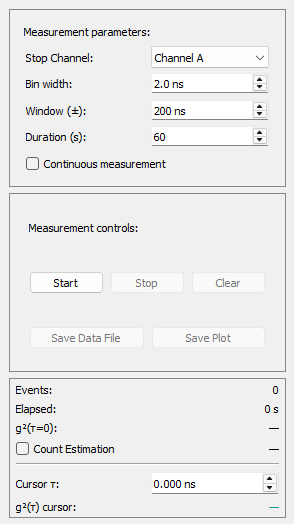
\includegraphics[width=3.06293in,height=5.4591in]{images/settings-before-measurements-2-02.png}
\label{fig:102}
\end{figure}

\hypertarget{perform-a-measurement-5}{%
\subsubsection{Perform a measurement}\label{perform-a-measurement-5}}

Once the desired configuration is selected, click the Start button to
begin the acquisition. While the measurement is running, the Stop
Channel, the Bin Width, the Window ($\pm$), the Duration, and the Continuous
measurement and Count Estimation checkboxes are locked and cannot be
changed. The g\textsuperscript{(2)}($\tau$) histogram is plotted live around
a reference line at g \textsuperscript{(2)} =1. At any point the user
can press Clear to reset the histogram, or Stop to end the measurement
before the configured duration elapses.

\begin{figure}[H]
\centering
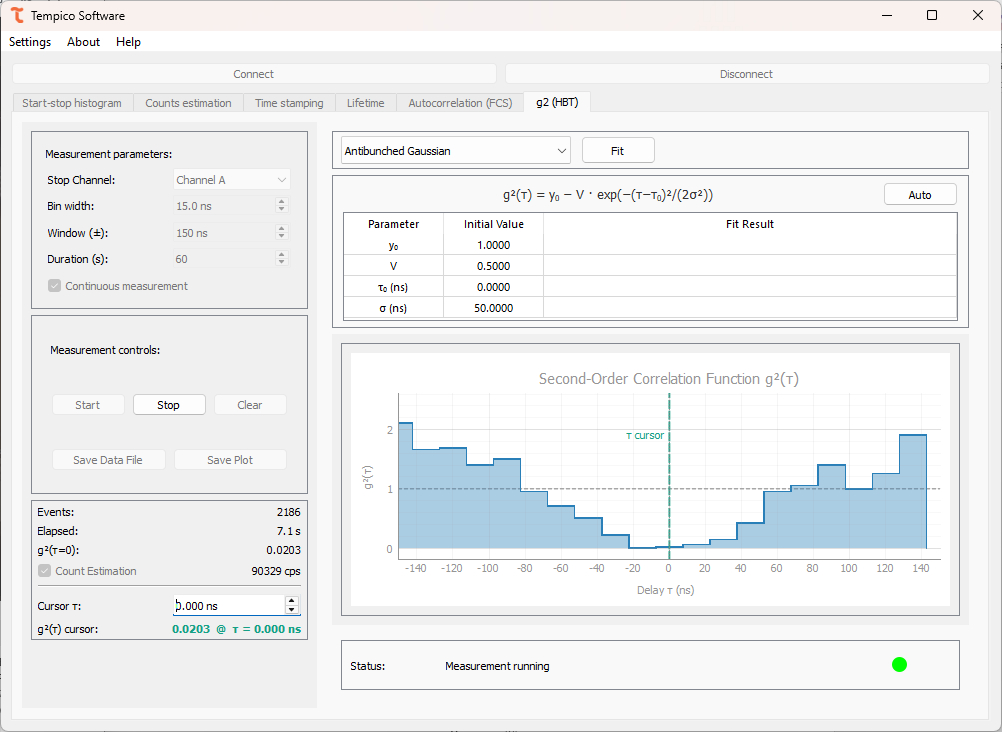
\includegraphics[width=5.89610in,height=4.30500in]{images/perform-a-measurement-5-01.png}
\label{fig:115}
\end{figure}

The panel below the settings reports the acquisition progress through
two values: Events, which indicates the number of valid stop events
detected on the selected channel since the measurement started, and
Elapsed, which indicates the elapsed time since the measurement started,
shown in seconds and, if applicable, against the total configured
duration. If Count Estimation was enabled before starting, this panel
also shows the estimated coincidence rate, in counts per second.

\begin{figure}[H]
\centering
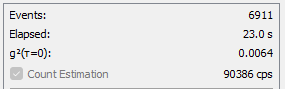
\includegraphics[width=2.97431in,height=0.92222in]{images/perform-a-measurement-5-02.png}
\label{fig:116}
\end{figure}

Next to this panel, the Status bar shows a colored dot together with a
short descriptive message, which the user should monitor throughout the
measurement. A grey dot indicates that no measurement is currently
running. A green dot indicates that the measurement is running normally,
with the message reporting the current number of events and elapsed
time. An orange dot indicates that a warning condition was detected: the
message ``No measurements in Start Channel'' means that the device is
not receiving any start pulses, while the message ``No measurements in
Stop Channel {[}A/B/C/D{]}'' means that no valid stop pulses are being
detected on the selected stop channel. If either warning persists, the
user should heck the corresponding cable connections and the signal
levels before continuing the measurement.

\begin{figure}[H]
\centering
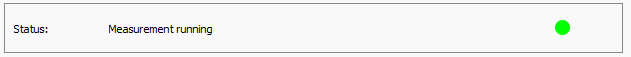
\includegraphics[width=6.13750in,height=0.55764in]{images/perform-a-measurement-5-03.png}
\label{fig:117}
\end{figure}

\begin{figure}[H]
\centering
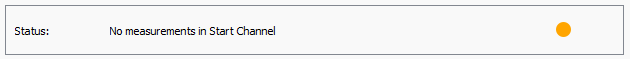
\includegraphics[width=6.13750in,height=0.57500in]{images/perform-a-measurement-5-04.png}
\label{fig:118}
\end{figure}

\hypertarget{post-measurement-1}{%
\subsubsection{Post-measurement}\label{post-measurement-1}}

\hypertarget{fitting-2}{%
\paragraph{Fitting}\label{fitting-2}}

Once the measurement finishes, the user can fit the
g\textsuperscript{(2)}($\tau$) histogram to one of five models available in
the fit model dropdown, located in the upper-right panel. Selecting
model updates the equation shown above the parameter table, which lists
an editable Initial value column and a read-only Fit result column. The
Auto button restores the initial guesses automatically suggested by the
software for the selected model.

Clicking Fit runs the fit and fills the Fit result column; the fitted
curve is then overlaid on the histogram. If a reliable value cannot be
estimated, the software reports ``nan'' for that parameter. Since the
quality of the fit depends on the initial guesses, the user is free to
edit them manually in the Initial value column before running the fit
again, or restore the software's suggested values with the Auto button.

\begin{figure}[H]
\centering
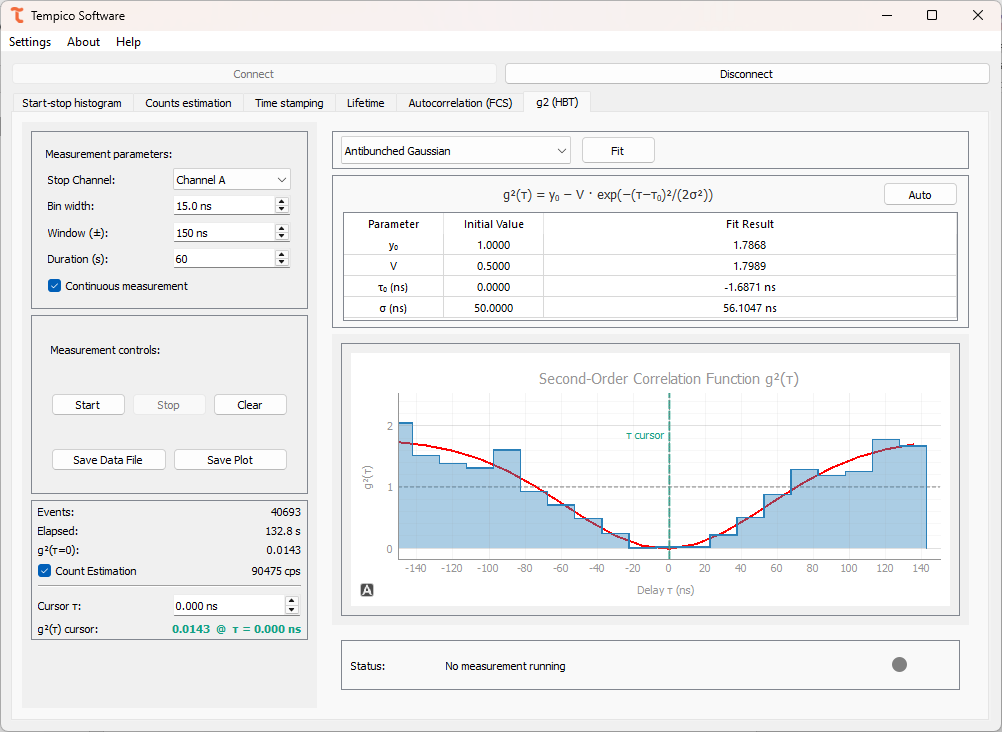
\includegraphics[width=5.69183in,height=4.15584in]{images/fitting-2-01.png}
\label{fig:119}
\end{figure}

\hypertarget{antibunched-gaussian}{%
\subparagraph{Antibunched Gaussian}\label{antibunched-gaussian}}

\[y_{0} - V \cdot \exp\left\lbrack - \frac{\left( \tau - \tau_{0} \right)^{2}}{2\sigma^{2}} \right\rbrack\]

Describes a dip in g\textsuperscript{(2)}($\tau$) with a Gaussian profile,
characteristic of a single-photon emitter with Gaussian-broadened timing
jitter. The fitted parameters are y\textsubscript{0}, the baseline level
far from $\tau$=0; V, the dip depth; $\tau$\textsubscript{0}, the position of the
dip, in ns; and $\sigma$, the width of the Gaussian dip, in ns.

\hypertarget{antibunched-lorentzian}{%
\subparagraph{Antibunched Lorentzian}\label{antibunched-lorentzian}}

\[y_{0} - V \cdot \frac{\left( \frac{\Gamma}{2} \right)^{2}}{\left( \tau - \tau_{0} \right)^{2} + \left( \frac{\Gamma}{2} \right)^{2}}\]

Describes a dip in g\textsuperscript{(2)}($\tau$) with a Lorentzian profile,
typical of a single emitter with an exponential excited-state lifetime.
The fitted parameters are y\textsubscript{0}, the baseline level; V, the
dip depth; $\tau$\textsubscript{0}, the position of the dip, in ns; and
\(\Gamma\), the full width at half maximum of the Lorentzian dip, in ns.

\hypertarget{bunched-gaussian}{%
\subparagraph{Bunched Gaussian}\label{bunched-gaussian}}

\[y_{0} - a \cdot \exp\left\lbrack - \frac{\pi\left| \tau - \tau_{0} \right|}{\tau_{c}}^{2}\  \right\rbrack\]

Describes a peak in g \textsuperscript{(2)} with an exponential profile,
also typical of bunched or thermal light. The fitted parameters are
y\textsubscript{0}, the baseline level; $\alpha$, the peak amplitude;
$\tau$\textsubscript{0}, the position of the peak, in ns; and
$\tau$\textsubscript{c}, the coherence time governing the width of the
Gaussian peak, in ns.

\hypertarget{bunched-lorentzian}{%
\subparagraph{Bunched Lorentzian}\label{bunched-lorentzian}}

\[y_{0} - a \cdot \exp\left\lbrack - \frac{\left| \tau - \tau_{0} \right|}{\tau_{c}}\  \right\rbrack\]

Describes a peak in g\textsuperscript{(2)}($\tau$) with an exponential
profile, also typical of bunched or thermal light but with a different
decay shape than the Gaussian case. The fitted parameters are
y\textsubscript{0}, the baseline level; $\alpha$, the peak amplitude;
$\tau$\textsubscript{0}, the position of the peak, in ns; and
$\tau$\textsubscript{c}, the coherence time governing the decay of the peak,
in ns.

\hypertarget{three-level-system}{%
\subparagraph{Three-level system}\label{three-level-system}}

\[1 - (1 + a) \cdot \exp\left\lbrack - \frac{\left| \tau - \tau_{0} \right|}{\tau_{1}} \right\rbrack + a \cdot \exp\left\lbrack - \frac{\left| \tau - \tau_{0} \right|}{\tau_{2}} \right\rbrack\]

Describes the g\textsuperscript{(2)}($\tau$) response of an emitter with an
additional metastable (shelving) state, combining an antibunching dip
with a bunching shoulder. The fitted parameter are a, the relative
amplitude of the bunching shoulder; $\tau$\textsubscript{0}, the position of
the feature, in ns; $\tau$\textsubscript{1}, the fast time constant
associated with the antibunching dip, in ns; and $\tau$\textsubscript{2}, the
slow time constant associated with shelving-state bunching, in ns.

\hypertarget{save-data-3}{%
\paragraph{Save data}\label{save-data-3}}

Once the measurement finishes, the Save Data File button is enabled.
Clicking it opens a dialog window where the user selects the file
format: .txt, .csv, or .dat. Two files are generated: one containing the
raw start-stop times recorded during the acquisition, and another with
the analyzed g \textsuperscript{(2)} curve, listing $\tau$ in nanoseconds and
the corresponding g \textsuperscript{(2)} value. Both files share a
header with the measurement window, the device model, the measurement
parameters, and the selected stop channel; if a fit was performed, the
fit model, its equation, and the resulting parameter values are also
included in the header.

\begin{figure}[H]
\centering
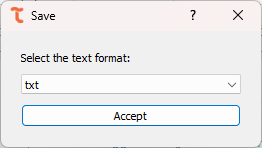
\includegraphics[width=2.8in,height=2.54in]{images/save-data-3-01.png}
\label{fig:120}
\end{figure}

\begin{figure}[H]
\centering
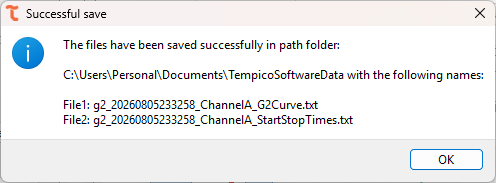
\includegraphics[width=5.16739in,height=1.90652in]{images/save-data-3-02.png}
\label{fig:121}
\end{figure}

\begin{figure}[H]
\centering
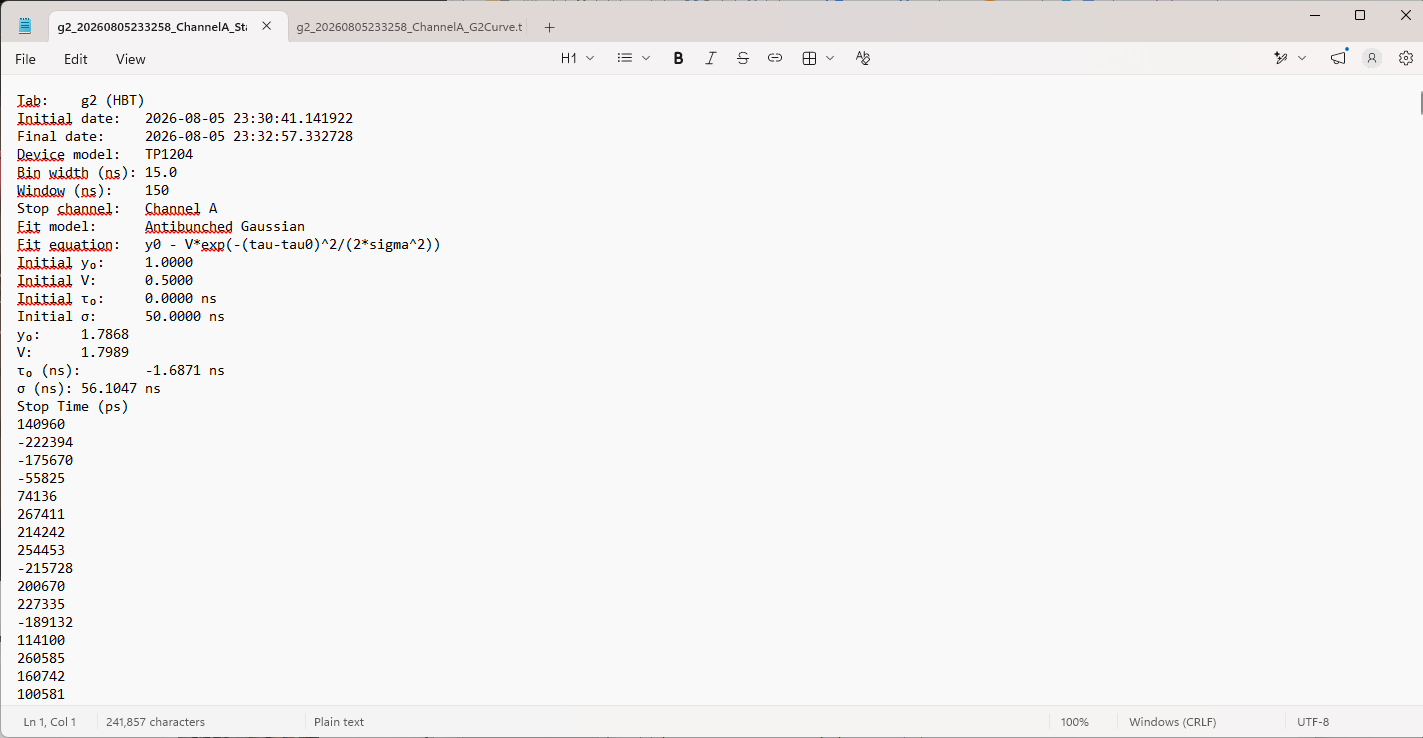
\includegraphics[width=6.13750in,height=3.18333in]{images/save-data-3-03.png}
\label{fig:122}
\end{figure}

\begin{figure}[H]
\centering
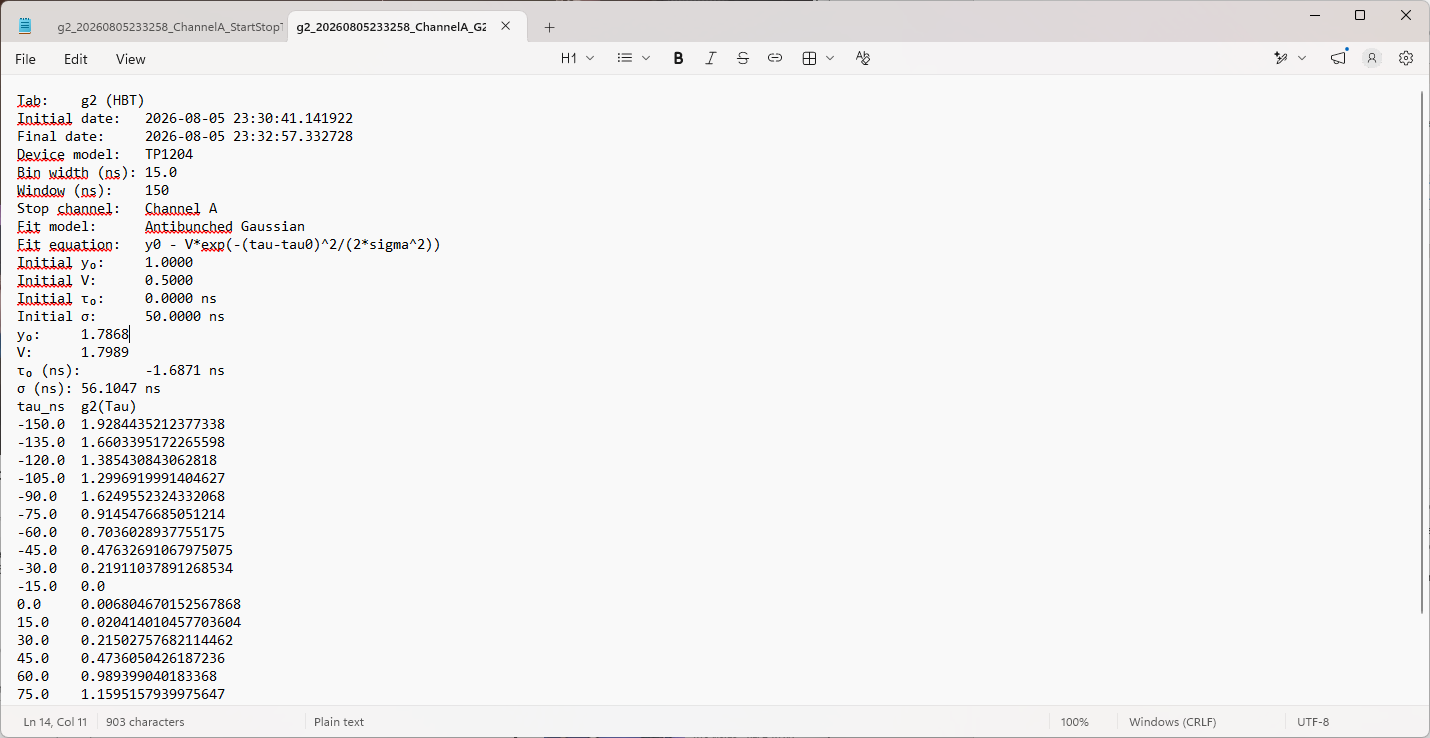
\includegraphics[width=6.13750in,height=3.16736in]{images/save-data-3-04.png}
\label{fig:123}
\end{figure}

Likewise, the Save Plot button exports the graph exactly as it appears
on screen, including the fitted curve if one was calculated. The
available formats are .png, .tiff, and .jpg. In both cases, once the
user selects the desired format and confirms, a confirmation window
appears indicating that the file was saved successfully and displaying
the path where it was stored.

\begin{figure}[H]
\centering
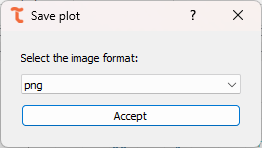
\includegraphics[width=3.0in,height=2.6in]{images/save-data-3-05.png}
\label{fig:124}
\end{figure}

\begin{figure}[H]
\centering
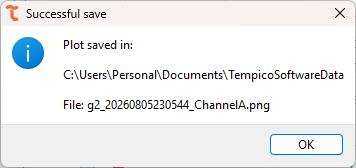
\includegraphics[width=3.71458in,height=1.75347in]{images/save-data-3-06.png}
\label{fig:125}
\end{figure}

\begin{figure}[H]
\centering
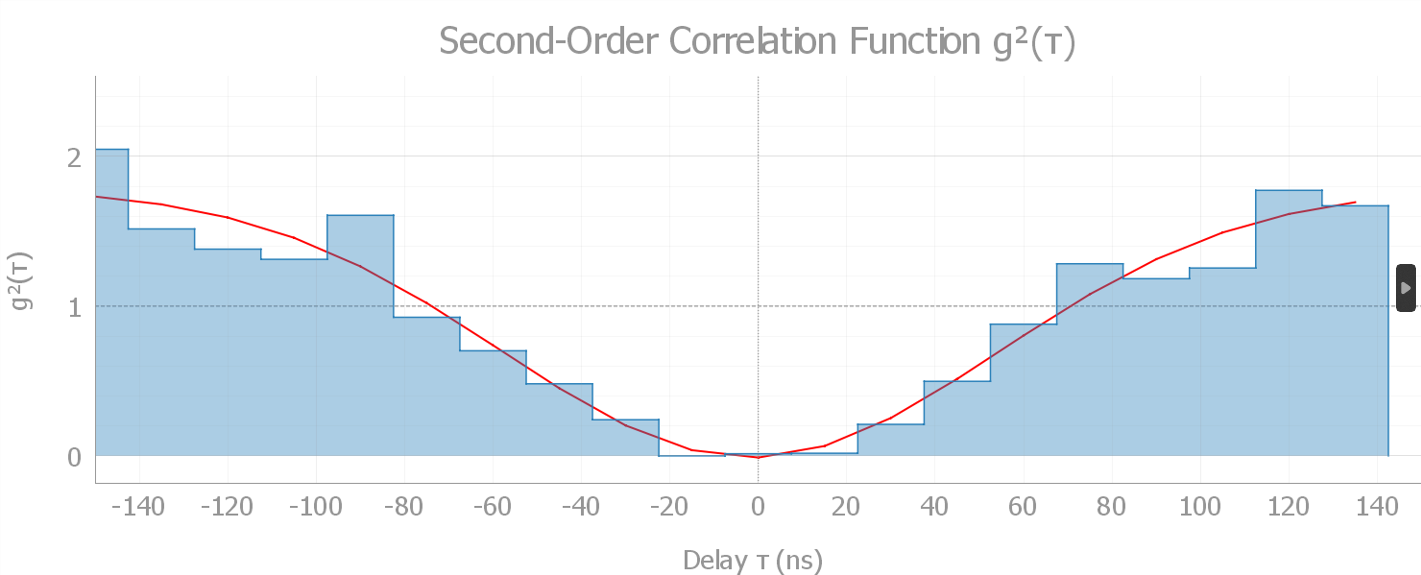
\includegraphics[width=6.03896in,height=2.48194in]{images/save-data-3-07.png}
\label{fig:126}
\end{figure}

\hypertarget{technical-documentation}{%
\section{Technical documentation}\label{technical-documentation}}

Tempico Software is open source, allowing access to the
software\textquotesingle s source code and developer documentation
through the GitHub platform. It also provides a guide to the code and
the creation of respective installers for each operating system.

\url{https://github.com/Tausand-dev/TempicoSoftware}

\hypertarget{drivers}{%
\section{Drivers}\label{drivers}}

Your computer may automatically download and install from the Internet
the required drivers once you connect your Tausand Tempico device to a
USB port. If you require to install them manually, they are available at
\url{https://www.tausand.com/downloads}.

\hypertarget{technical-support}{%
\section{Technical support}\label{technical-support}}

For technical support, contact us at
\href{mailto:support@tausand.com}{\nolinkurl{support@tausand.com}}.

Visit our website to check for the latest documentation and software
releases.

\href{http://www.tausand.com}{www.tausand.com}

\end{document}